\documentclass[a4paper,11pt]{report}
\usepackage{graphicx,booktabs,apacite}
\usepackage{amsmath,amsfonts}
\usepackage{comment}
\usepackage{multirow}
\usepackage{url}

% FILL OUT THE DETAILS BELOW:
\author{Sameeksha Aggarwal}
\title{The Influence of Company Name Fluency on Stock Market Performance}
% \date{An optional custom date, the default is today}
\newcommand{\studentnumber}{560575}
\newcommand{\program}{Business Analytics and Quantitative Marketing}
\newcommand{\supervisor}{Flavius Fransincar}
\newcommand{\secondassesor}{Wendun Wang}

\usepackage[british]{babel} % Use British English
\usepackage[onehalfspacing]{setspace} % Increase line spacing
\usepackage[margin=2.5cm]{geometry} % Modify margins


\begin{document}

\begin{titlepage}
\makeatletter
\begin{center}
	\textsc{Erasmus University Rotterdam}
	\par \textsc{Erasmus School of Economics}
	\par Master Thesis \program

	\vfill \hrule height .08em \bigskip
	\par\huge\@title\bigskip
	\par\Large\@author\,(\studentnumber)\bigskip
	\hrule height .08em\normalsize
	
	\vfill
	
\includegraphics[width=\textwidth,height=0.15\textheight,keepaspectratio]{eur (1).png} 
	\vfill
	
	\begin{tabular}{ll}
		\toprule
		Supervisor: & \supervisor\\
		Second assessor: & \secondassesor\\
		Date final version: & \@date\\
		\bottomrule
	\end{tabular}
	
	\vfill
	The content of this thesis is the sole responsibility of the author and does not reflect the view of the supervisor, second assessor, Erasmus School of Economics or Erasmus University.
\end{center}
\makeatother
\end{titlepage}

\begin{abstract}
The ease with which investors process and remember a company’s name can subtly shape their perceptions and decisions, influencing market outcomes beyond traditional financial metrics. In this study, a name fluency score is constructed using multiple word attributes using a neural network. The model demonstrates superior predictive accuracy compared to baseline benchmarks in out-of-sample tests, effectively capturing complex linguistic patterns. This trained model is applied to financial data spanning from 1980 to 2024 to generate company name fluency scores. The extrinsic effects of these scores are then examined using fixed-effect panel regression, Difference-in-Difference analysis focused on company name changes, and a cross-sectional regression. Panel regressions reveal that higher name fluency is positively and significantly associated with firm valuation, suggesting that easier-to-process names enhance long-term market value. Conversely, fluency exhibits a negative relation with liquidity and performance, implying that while fluent names improve perceived value, they do not necessarily translate into higher trading activity or short-term returns. The Difference-in-Difference analysis further confirms that companies undergoing a name change experience significant increases in valuation, liquidity, and performance relative to firms that retain their names, highlighting the short-term benefits of rebranding. Cross-sectional regression finds fluency positively associated with valuation and liquidity but negatively linked to long-term financial performance. 

\end{abstract}

\newpage
\tableofcontents

\newpage
\listoffigures

\newpage
\listoftables

\chapter{Introduction}

Names are a fundamental part of a person's identity. They embody individuality while also serving as a social bond that connects a person to their family and heritage, often expressed through a single name\cite{name1}. The same applies to a company's name, as it often serves as a strong signal to the public about the identity and nature of the business. \citeA{impor_name1} tested the effectiveness of short and snappy brand names. The study found that shorter brand names are processed more quickly, largely due to their higher frequency and monosyllabic nature in the English language, and are commonly linked to more basic or generic brands. In contrast, longer and more unique brand names help create a distinct identity in people's minds, making them well-suited for luxury brands by enhancing memorability and setting them apart. \citeA{impor_name2} highlighted the challenges of using initials for company names as opposed to full names. They also show that brands with suggestive or meaningful names lead to higher interaction with people. Another key insight from the research is the importance of choosing a brand name that evokes familiar real-world meanings, even if it does not directly reference specific product attributes or benefits. By extension, such familiarity can create a bias that shapes how investors evaluate and respond to the company. 

Furthermore, using words with negative connotations can create a bigger impact on the audience, as shown by \citeA{impor_name3}. Brand names like ``Poison'' perfume or ``Monster'' energy drinks are better recognised compared to non-negative brands, but they do have a detrimental influence on the products and brand image as the negative influence potentially increases. Although a company's name plays a crucial role in shaping consumer perceptions and preferences, its influence extends beyond the market. It can affect investor behaviour by shaping expectations, signalling firm identity, and affecting perceived credibility.

Traditional finance theories, such as the Efficient Market Hypothesis, assume that investors are fully rational and markets always reflect all available information \cite{cog_bias_finance}. However, numerous empirical anomalies, such as momentum effects (stocks that have performed well in the past tend to continue to perform well in the near future, and those that have performed poorly tend to continue underperforming), asset bubbles, and excessive trading challenge this assumption. Behavioural finance offers an alternative perspective by recognising that investors often rely on heuristics and are subject to cognitive biases when making decisions \cite{cog_bias_finance1}. Cognitive biases can lead to systematic deviations from rational behaviour, which in turn affects pricing, liquidity, and market stability. Studies including those by \citeA{cog_bias_finance2} have shown that overconfidence bias leads to excessive trading, while \citeA{cog_bias_finance3}'s Prospect Theory demonstrates how loss aversion distorts investment decisions. Understanding these biases is crucial because they not only affect individual investors' outcomes but also have broader implications for market efficiency, asset mispricing, and regulatory policy \cite{cog_bias_market}.

While many biases exist, company name fluency is particularly important because it directly influences initial investor attention and perception. The company's name is often the first piece of information processed, and first impressions are known to heavily bias subsequent judgments \cite{why_bias}. Recent studies suggest that fluent names, those that are easier to pronounce, shorter, or more familiar, elicit positive emotional reactions and lead to favourable evaluations due to processing ease for the investors \cite{why_bias2}. Some of these biases stem from alphabetical ordering of company names \cite{alpha}, fluency of company names \cite{fluency, fleuncy2_main}, or memorability of the names \cite{memory}. \citeA{investor_behave} show that private investors are more prone to behavioural biases like alphabetical ordering, company name fluency, and memorability than institutional investors, hence effecting their investing behaviour. These biases can sway the investors in investing in companies with better-sounding names. An example of a fluent brand name is ``PayPal'', the name clearly communicates the company's purpose, making it intuitive and appealing for investors. In contrast, ``Fiserv'', another company in the same industry, has a name that does not immediately convey what the company does, making it less intuitive for investing. 

All of the above biases can be summed up as processing fluency. It can be defined as the subjective experience of ease with which the information is processed, driven by speed and accuracy of the stimulus processing, independent of the stimulus content \cite{def_fluency}. It is hypothesized that companies with more fluent names, those that are easier to process and more familiar-sounding, are associated with higher valuations, greater liquidity, and better stock performance compared to companies with less fluent names. This research offers valuable insights for companies seeking to better understand investor behaviour and strategically leveraging cognitive biases to attract greater investment. Simultaneously, it helps investors become more aware of their own behavioural biases and how it may shape their investment decisions.

Prior studies have shown that private investors are particularly sensitive to superficial cues such as alphabetical ordering, name fluency, and memorability, while institutional investors are relatively less affected \cite{memory2}. However, while some research has established the importance of name fluency, there is limited investigation into how name fluency systematically affects key stock characteristics such as valuation, liquidity, and performance over extended periods. Many works explore the topic of fluency primarily through experimental setups or basic statistical methods, which often lack a robust justification for the underlying fluency score. This paper introduces a deep learning model to provide a data-driven and systematic approach to estimating word fluency based on standardized linguistic features. By doing so, it moves beyond traditional techniques and offers a more objective and scalable method for assessing fluency. Hence, this paper aims to enhance the finance field by incorporating a machine learning model to compute a fluency score and subsequently applying panel regression to examine its statistical significance in relation to firm-level outcomes.

An important research gap exists in understanding how corporate name changes over time influence investor perception and stock performance. Companies may change their names to distance themselves from negative reputations, align with positive associations, or signal strategic shifts such as expanding or narrowing their business focus \cite{change_in_name}. Such changes can be a powerful tool to shape investor sentiment. Additionally, there is a need to explore how a company’s performance aligns with the implications conveyed by its name, suggesting that a more fluent new name could be associated with improved performance and greater liquidity compared to the previous name.

Additionally, previous fluency measures have primarily relied on basic attributes like length or how English the name is, whereas expanding the fluency score to incorporate additional characteristics such as repetition, prototypicality, and phonetic appeal could provide a more nuanced understanding of how company names influence investor behaviour and market performance. Addressing these aspects is crucial, as it offers deeper insights into how linguistic features can have persistent and systematic financial effects, influencing not only individual investment decisions but also broader market outcomes.

Therefore, this paper aims to investigate whether the fluency of a company's name significantly influences its stock valuation, liquidity, and performance across a large panel of firms and over an extended period with an informative fluency score. The research question is: \\

\textit{Does a company's name fluency have a significant effect on the characteristics of its stock?}\\

The selected stock characteristics provide a comprehensive overview of the company and offer valuable insights into its market perception and financial standing. The fluency score is calculated using a deep learning model and the frequency of the words along with other characteristics like alphabetical order, word length, spell check, and symmetry. The frequency with which a word is encountered serves as a reliable proxy for its fluency, as words that are more commonly seen or heard tend to be more easily processed and recalled. Repeated exposure strengthens mental associations, facilitating quicker comprehension and cognitive accessibility \cite{open2009}. Once the fluency score is computed for each company, a panel regression with fixed effects is conducted using firm-level stock data to analyse the effect of name fluency on selected stock characteristics. Short-term effects of the name change are explained using a Difference-in-Difference analysis and finally a cross-sectional regression is used to explain the long term effects of having a more fluent name.  

The code is written in Python using TensorFlow and Keras for the neural network modelling of company name fluency, while the fixed-effect panel regression, Difference-in-Difference analysis and, cross-sectional regressions are implemented in Stata. Both data and code are made freely available at: \url{https://github.com/sameekshaagg/FluencyOnStock}. The dataset contains 28,320 companies, with names and quarterly stock characteristics collected over the period 1980–2024. The Python scripts include preprocessing, model training, and fluency score generation, while Stata scripts handle the regression analyses and robustness checks, ensuring full reproducibility of the results.

The paper is structured as follows. The previous research on the effect of fluency of company name on stocks and use of deep learning models in linguistic features is discussed in Chapter \ref{sec:lit}, followed by the description of the dataset in Chapter \ref{sec:data}. In Chapter \ref{sec:neural_network}, the neural network model along with different regression are outlined. The results are analysed in Chapter \ref{sec:results}. Last, in Chapter \ref{sec:conclusion}, the significance of the findings, the limitations, and future research directions are given. 

\chapter{Related Work} \label{sec:lit}
This chapter reviews the relevant literature. Section \ref{Behave} examines prior research in the field of behavioural finance, highlighting the importance of company names and laying the groundwork for the features used to construct the fluency score. Section \ref{deep_model} explores various deep learning approaches used to model fluency scores and analyse linguistic characteristics.

\section{Behavioural Finance} \label{Behave}
A company name is an important characteristic for a company as it conveys information about the company's quality, mission statement, and identity to investors. In a study by \citeA{brandidentity}, brand names with positive attributes are typically favoured more and are much easier to recall compared to non-meaningful brand names. Though with repeated exposure it is observed that there is significant improvement for non-meaningful names compared to meaningful names. The authors also highlight the benefits to managers to use a meaningful name and for companies with larger promotional budgets to use non-meaningful brand names as a viable alternative. The survey results suggest that company names influence respondents' perceptions and affect how favourably a company is viewed based solely on its name.

\citeA{brandidentity2} show that a strong brand name can produce strong brand associations contributing to a brand positioning in an investor's mind. A suggestive brand name facilitates the recall of the company name but at the same time it can be difficult to expand the product range if the name is too specific. It is hard to say if a company name is a strong word or influential, hence the fluency of the company name can be used to process the effect of the company's name on the investor's behaviour. \citeA{fluencyfeatures} demonstrate that the factors which enhance the ease of processing a stimulus leads to more positive emotional responses from participants, compared to stimuli that are more difficult to process. Their study focuses specifically on perceptual fluency, which refers to the ease with which the physical features of a stimulus are recognized. Factors such as the amount of information, symmetry, clarity, and repetition all contribute to perceptual fluency, shaping how effortlessly a stimulus is processed. In particular, the amount of information is emphasized as a critical component influencing processing ease \cite{amtinfo2}. 

\subsection{Fluency Effect}
\citeA{fluencyfeatures} lays the psychological foundation of processing fluency and focuses on different stimuli which can give rise to fluency. These stimuli include amount of information, symmetry, contrast, and clarity. This was further built on by \citeA{why_bias2} who introduced the idea of fluency score specifically related to company names. They conducted three studies wherein the first study was used to understand the effect of simple versus complex company names. The second study investigates how the fluency of a company name affects investor perceptions at different time horizons, ranging from 1 day to 1 year. The first two studies show that a company's name does influence people's prediction about the company's share performance. A third study addressed potential biases introduced by foreign names or buzzwords by using stock tickers instead of company names. The results matched the first two studies where the more pronounceable tickers were favoured by the investors.

Another research by \citeA{oppen1} further support that familiarity and fluency are able to influence people with valuations. Experiments showed that participants perceived familiar currencies as having greater purchasing power compared to unfamiliar currencies. The results from the experiment confirmed that familiar stimuli are more valuable because they can be processed more fluently. This concept can also be extended to stocks and investor behaviour, as more fluent company names may enhance investor understanding and familiarity, fostering a positive bias toward investing in the company, creating cognitive biases among investors and influencing market outcomes. Through different experiments, \citeA{name_fleuncy} examine the effect of company name fluency on expected stock returns across different conditions. The study finds that investors expect higher returns from companies with fluent names, even when told that names are not real. The fluency effect remains significant across various conditions but weakens when more meaningful information is provided. It is driven by both conscious and unconscious processes, and its persistence may be explained by information overload, which leads investors to rely on simple heuristics like name fluency. 


\subsubsection{Alphabetical Order}
Some of the research done in this field is based on specific biases and how they impact the investor behaviour. One such bias is the alphabetical bias, both \citeA{AlphabeticBias} and \citeA{alpha} show that alphabetical bias exists and that it affects trading activity and liquidity of the companies. \citeA{alpha} focused their research on the effect of alphabetically bias and found early alphabet stocks are traded more frequently than later alphabet stocks. The effect has increased over time with the advent of the Internet. This effect is concentrated in stocks dominated by individual investors and the reasoning behind this behaviour is due to satisficing (investors may prefer to make decisions that feel more familiar rather than engaging in complex decision-making processes) and status quo bias (individuals tend to stick with the current situation due to stability). 

\citeA{AlphabeticBias} explore the effect of alphabetical bias within the stock market using predictive panel regressions. Their results highlight that stocks appearing earlier alphabetically get more investor attention leading to higher trading volume and greater liquidity. Moreover, companies with shorter, simpler, and easier-to-pronounce names gain more attraction from the investors. Due to the limited attention and heuristics preprocessing, the investors are not able to process all the available information. The authors also focus on name changes, international stock markets, and mutual funds to further back their results of alphabetical bias. 

The above effect is prevalent in saving plans like 401(K) investing, too. \citeA{alpha2} show that funds at the beginning of an alphabetically sorted list receive greater allocation compared to funds toward the end of the list. Their research support the alphabetical bias in both small and large choice sets. The bias grows as the number of funds in the plan increases, similar to the findings of \citeA{AlphabeticBias}, where investors are unable to process all the available information effectively.

\subsubsection{Memorability}
Another factor of fluency is memorability, if a person can remember the word then they lean towards it compared to an unfamiliar word. \citeA{memory2} study the relationship between brand perception and companies. It found that brand awareness plays a more crucial role than brand image, and individual investors tend to favour companies with recognizable products. Hence, it is possible to influence the investors to hold a company's stock if the brand perception is memorable enough. Using multivariate regression and portfolio analysis, \citeA{memory} show that increased firm visibility among investors results in a larger base of individual and institutional investors, enhanced liquidity, and improved company performance. This effect is stronger on common shareholders compared to institutional shareholders, but nonetheless significant for both. Therefore, developing a memorable or strong brand image can influence investors, making them more familiar with the brand and, as a result, creating a bias.

Similarly, \citeA{green_fund} demonstrate that funds that are changing their names to a substantiality related name, observe an increase in fund flows and a rise in portfolio turnover. The authors demonstrate that the investors tend to prefer names associated with sustainability, such as ``Green'' or ``Eco'' when choosing mutual funds on sustainable investments. Another research on changing names is done by \citeA{dotcom} who investigated the effect of changing a company's name to a dot-com name during the dot-com bubble. They use time series along with panel data to show that a change in name leads to a significant positive effect on the stock price, with the effect being more prominent for the firms with lower prices and volumes. Another key finding from the work is that the positive returns associated with the name change are not short-lived and with no evidence of a post-event negative effect. This suggests that aligning a company's name with current trends can help attract investors and capitalize on benefits.

\subsubsection{Syllables}
An important factor of a name is its ease of pronunciation, as well as features like repetition, which can make it easier for people to remember. \citeA{sylla1} use experiments to show that participants lean towards names with fewer syllables and deem them as less risky and more trustworthy compared to difficult-to-pronounce names, due to heightened perceptions of novelty. This effect is consistent across contexts like food safety and entertainment, and is not driven by emotional responses but rather by how novel the stimuli seem. The findings suggest that various factors affecting processing fluency can significantly shape risk perception. 

Through experiments, \citeA{sylla2_sound} are able to prove that certain sounds can influence consumer perception and preferences. This research, conducted in the field of marketing and brand names, demonstrates that the phonetic symbolism effect is real. It shows that the sound of words can convey meaning and influence consumer judgments. This effect is further explored in relation to vowel and consonant sounds. Front vowels, such as the ``ee'' in ``beet'', are commonly associated with qualities like smallness, weakness, or pleasantness, while back vowels, like the ``oo'' in ``boot'', tend to be linked to perceptions of largeness, strength, or unpleasantness. Similar associations are observed with certain consonants, highlighting how the sound structure of a word can subtly influence our emotional or physical perception, even without contextual meaning.

\citeA{birds_repe} conducted a between-subjects study in which participants rated the accuracy of aphorisms. In this study some participants were warned to separate poetic features from content, while others received no such instruction. They were able to identify the rhyme-as-reason effect, where rhyming aphorisms are perceived as more accurate than non-rhyming equivalents due to their increased processing fluency. However, this effect weakens when participants are explicitly instructed to separate poetic form from the underlying meaning, suggesting that rhyme can bias judgments of truth unless critical thinking is prompted. This implies that investors may have a more positive perception of company names that rhyme. All these factors can be used in the fluency score to get an overview of the different aspects of words which can create bias to an investor. 

\subsubsection{Combination of Factors}
Some recent literature has focused on combining different aspects of literary factors to create the fluency score. One such research is by \citeA{fleuncy2_main}, who study the relationship between company names and investor behaviour by creating a summed-up fluency score based on three aspects: a length score, an Englishness score (Travers and Olivier, 1978), and a grammar check score. They use panel regressions to analyse how company name fluency influences breadth of ownership, liquidity, and firm value, with a focus on retail and mutual fund investors. The study finds that closed-end funds with fluent names trade at higher premiums relative to their net asset values compared to less fluent funds. Additionally, companies with more fluent names attract investors and experience higher turnover.

A more recent research by \citeA{company_name_montone} uses Fama-MacBeth and panel regression with year fixed effects to analyse the relationship between the company name fluency and stock returns. Following the methodology of \citeA{fleuncy2_main}, the authors construct a composite fluency score. They further incorporate interaction terms between fluency, sentiment, and firm size to examine the conditional relationship between fluency and stock returns. The results show that the effect of fluency on stock returns is positive and significant, but limited to small-cap stocks. Additionally, the positive impact of fluency on returns is significant for stocks with high sentiment, but not for those with low sentiment. The study also concludes that companies with fluent names enjoy higher valuations, excess returns, and stronger operating performance, while naive investors tend to overlook the valuable information embedded in name fluency.

\citeA{investor_behave} studies the impact of name based biases on stock trading between institutional and individual investors. The study is conducted using regression and multivariate testing. Some of the components focused in this study are: alphabetical order, fluency, and memorability. When creating a distinction between investors, it was found that individual investors rely heavily on name-based heuristics, whereas institutional investors appear immune to alphabetical order and name-fluency bias. Consequently, more recent studies have begun integrating various aspects of names to develop a composite fluency score, aiming to better capture their overall impact.

\section{Deep Learning for Name Fluency} \label{deep_model}
In recent years, the concept of name fluency has gained attention for its influence on consumer behaviour, investor perception, and company performance. Traditionally studied through linguistic and psychological lenses via surveys and experiments, name fluency is now being explored through statistical methods and regressions. Though many researchers have combined different aspects of company name to create a fluency score, not much research is done with deep learning models to compute the fluency score. With advances in natural language processing and deep learning, researchers are beginning to develop models that can quantify and predict sentiment related words which can be adapted for fluency, too. 

\subsection{Fluency and Sentiments}

Name fluency is an exposure effect that makes people feel more comfortable or familiar, which in turn encourages them to invest in the company. Once such example is discussed by \citeA{why_bias2} where one predicts that ``Barnings'' will have a higher future returns compared to ``Xagibdan'' based on the fluent names of the company. Therefore, gaining a deeper understanding of fluent names can enhance our insight into the sentiments they evoke and how these sentiments influence people’s perceptions and decisions. Sentiment analysis is a study to understand the language used to express human opinions, emotions, sentiments, and mood through big data techniques \cite{sentiment_def}. A sentence has multiple words and each word has a sentiment attached to it, as shown in the example below. \\

\textit{The movie was quite cheerful, but the protagonist appeared lugubrious.}\\

The above sentence contains words ``cheerful'', ``movie'', and ``lugubrious'' which express the context of the sentence, in this case known as polarity. In the above example, ``cheerful'' has a positive polarity, ``movie'' has neutral, and ``lugubrious'' has negative polarity. This captures the sentiment of the sentence as intended by the sender, but this research focuses on understanding the reader's experience. The emphasis is on the ease with which a word is processed by the reader, independent of its meaning. The fluency score reflects how easily the reader can understand the company name. For example, ``cheerful'' is easier to process compared to ``lugubrious'', so a name with ``cheerful'' in it would be  preferred over one with ``lugubrious''. This is due to the familiarity of the word which is determined using a deep learning model, in our research due to the versatility of such a model. 


\subsection{Deep Learning Model}
Deep learning is a subfield of machine learning that uses neural networks with multiple layers to automatically learn hierarchical features from data. These models excel in tasks such as natural language processing and speech recognition by processing raw data through layers of neurons, adjusting weights via back-propagation to minimize error \cite{dl, dl1}.

Deep learning models are quite popular in classifying emotions. Once such research is done by \citeA{dl_emotions} where pre-trained language models like BERT and USE are fine-tuned using emotion-labelled data to classify emotions more accurately. BERT is a model that understands word meaning using context from both directions in a sentence, while USE converts entire sentences into meaningful vector representations for language tasks. These models allow for transfer learning, feature extraction, and layer freezing/unfreezing help improve learning efficiency and model performance. They can leverage prior linguistic knowledge, reduce training time, and perform well even with limited labelled data, making emotion classification more effective and scalable. In addition, they are able to achieve high accuracy of 91\% in multi-class emotion classification and the fine-tuning on the model allows it to be robust and highly effective. 

Similarly, \citeA{ensemble_deep} utilize various deep learning models, including RNN-based (handle sequential data by maintaining memory of previous inputs), CNN-based (captures local patterns in data), and transformer-based (uses self-attention to process entire sequences in parallel) architectures, along with an ensemble learning approach (combines predictions from multiple models to improve accuracy and robustness) to classify emotions in English conversations. The study compares model performance, showing that transformer-based models outperform RNN-based ones. Additionally, the ensemble approach yields better results than individual models, highlighting that combining different inputs and classifiers enhances overall performance. \citeA{transformerML} introduced the transformer model, which has become foundational in natural language processing tasks. Their main focus is on translations such as English-to-German and English-to-French. The transformer is able to outperform models based on recurrent and convolutional layers. Moreover, one the biggest advantage of the transformer is the faster training speed due to parallelisation than compared to other models. This model can be adapted to analyse the linguistic features of the company names and assess their fluency based on the phonetic and semantic patterns, however, this aspect is not addressed in the current study and represents a potential avenue for future research.

Deep learning has proven effective in natural language processing, classifying emotions and speech recognition, but not much research is done on fluency of company names. These methods might seem to be ad hoc, yet deep learning is similar to neuroscience learning \cite{ML_neuro2}. \citeA{ML_neuro} shows that the brain performs learning by optimizing multiple internal cost functions and using a variety of biologically grounded mechanisms. These include processes functionally similar to optimization techniques like back-propagation. These mechanisms are not static, they are shaped and fine-tuned over time to support flexible, adaptive learning. Moreover, the brain appears to use a bootstrapped developmental approach, where early-learned capabilities provide the foundation for more complex learning later on. This structured layering of learning objectives mirrors techniques in machine learning where simpler tasks are learned first to enable mastery of more complex functions. Hence, deep learning can be used to mimic patterns of brain activity involved in language processing and perception, allowing it to generate a fluency score for company names.

\chapter{Data} \label{sec:data}
This chapter introduces the data that is used for the training of the proposed deep learning model and the control variables used in the evaluation of the fluency score. First in Section \ref{sec:lexicon}, we present an extensive list of English words which is referred as \textit{lexicon}. Next, in Section \ref{sec:frequency}, we introduce a \textit{frequency list} of English words which is used to train, validate, and test the deep learning model. In Section \ref{sec:company_info}, a \textit{list of company names} is given in order to be used by the deep learning model to predict the fluency scores and finally the \textit{control variables} are provided to be used for evaluation of fluency prediction.

\section{Lexicon} \label{sec:lexicon}
The lexicon is a curated collection of English words used to generate features for the deep learning model. The lexicon data used in this research combines two English word datasets online. The first dataset is obtained from the words module of the Natural Language Toolkit (NLTK) library (\url{https://www.nltk.org/nltk_data}) and contains approximately 236,000 words. The second dataset is from the English-words library (\url{https://pypi.org/project/english-words}), with around 340,000 words. These two datasets are merged, with duplicates, single-letter words, and words containing special characters removed. To standardize the list, all words are converted to lowercase, lemmatized, and only unique lemmas are retained. This preprocessing step is crucial because the raw, uncleaned list contains multiple inflected forms of the same word (such as plurals, different tenses, or derived forms), which can artificially inflate the frequency counts and introduce bias. As a result, the final lexicon contains 253,825 distinct words. 

\section{Frequency List} \label{sec:frequency}
The dataset used to train our machine learning model is a frequency list, which ranks words based on how often they appear in a given corpus. Each word is labelled with its frequency, which we treat as a proxy for its processing fluency. This frequency serves as our target variable. The goal is to train a machine learning model that accurately predicts this target based on various features of the word. The frequency list is obtained from Google Web Trillion Word Corpus via Linguistic Data Consortium (\url{https://norvig.com/ngrams}). This list consists of 9244879 words but words with special characters and single letters are removed. This reduces the size of the list to 9013878 words. 

\begin{figure}[h!]
    \centering
    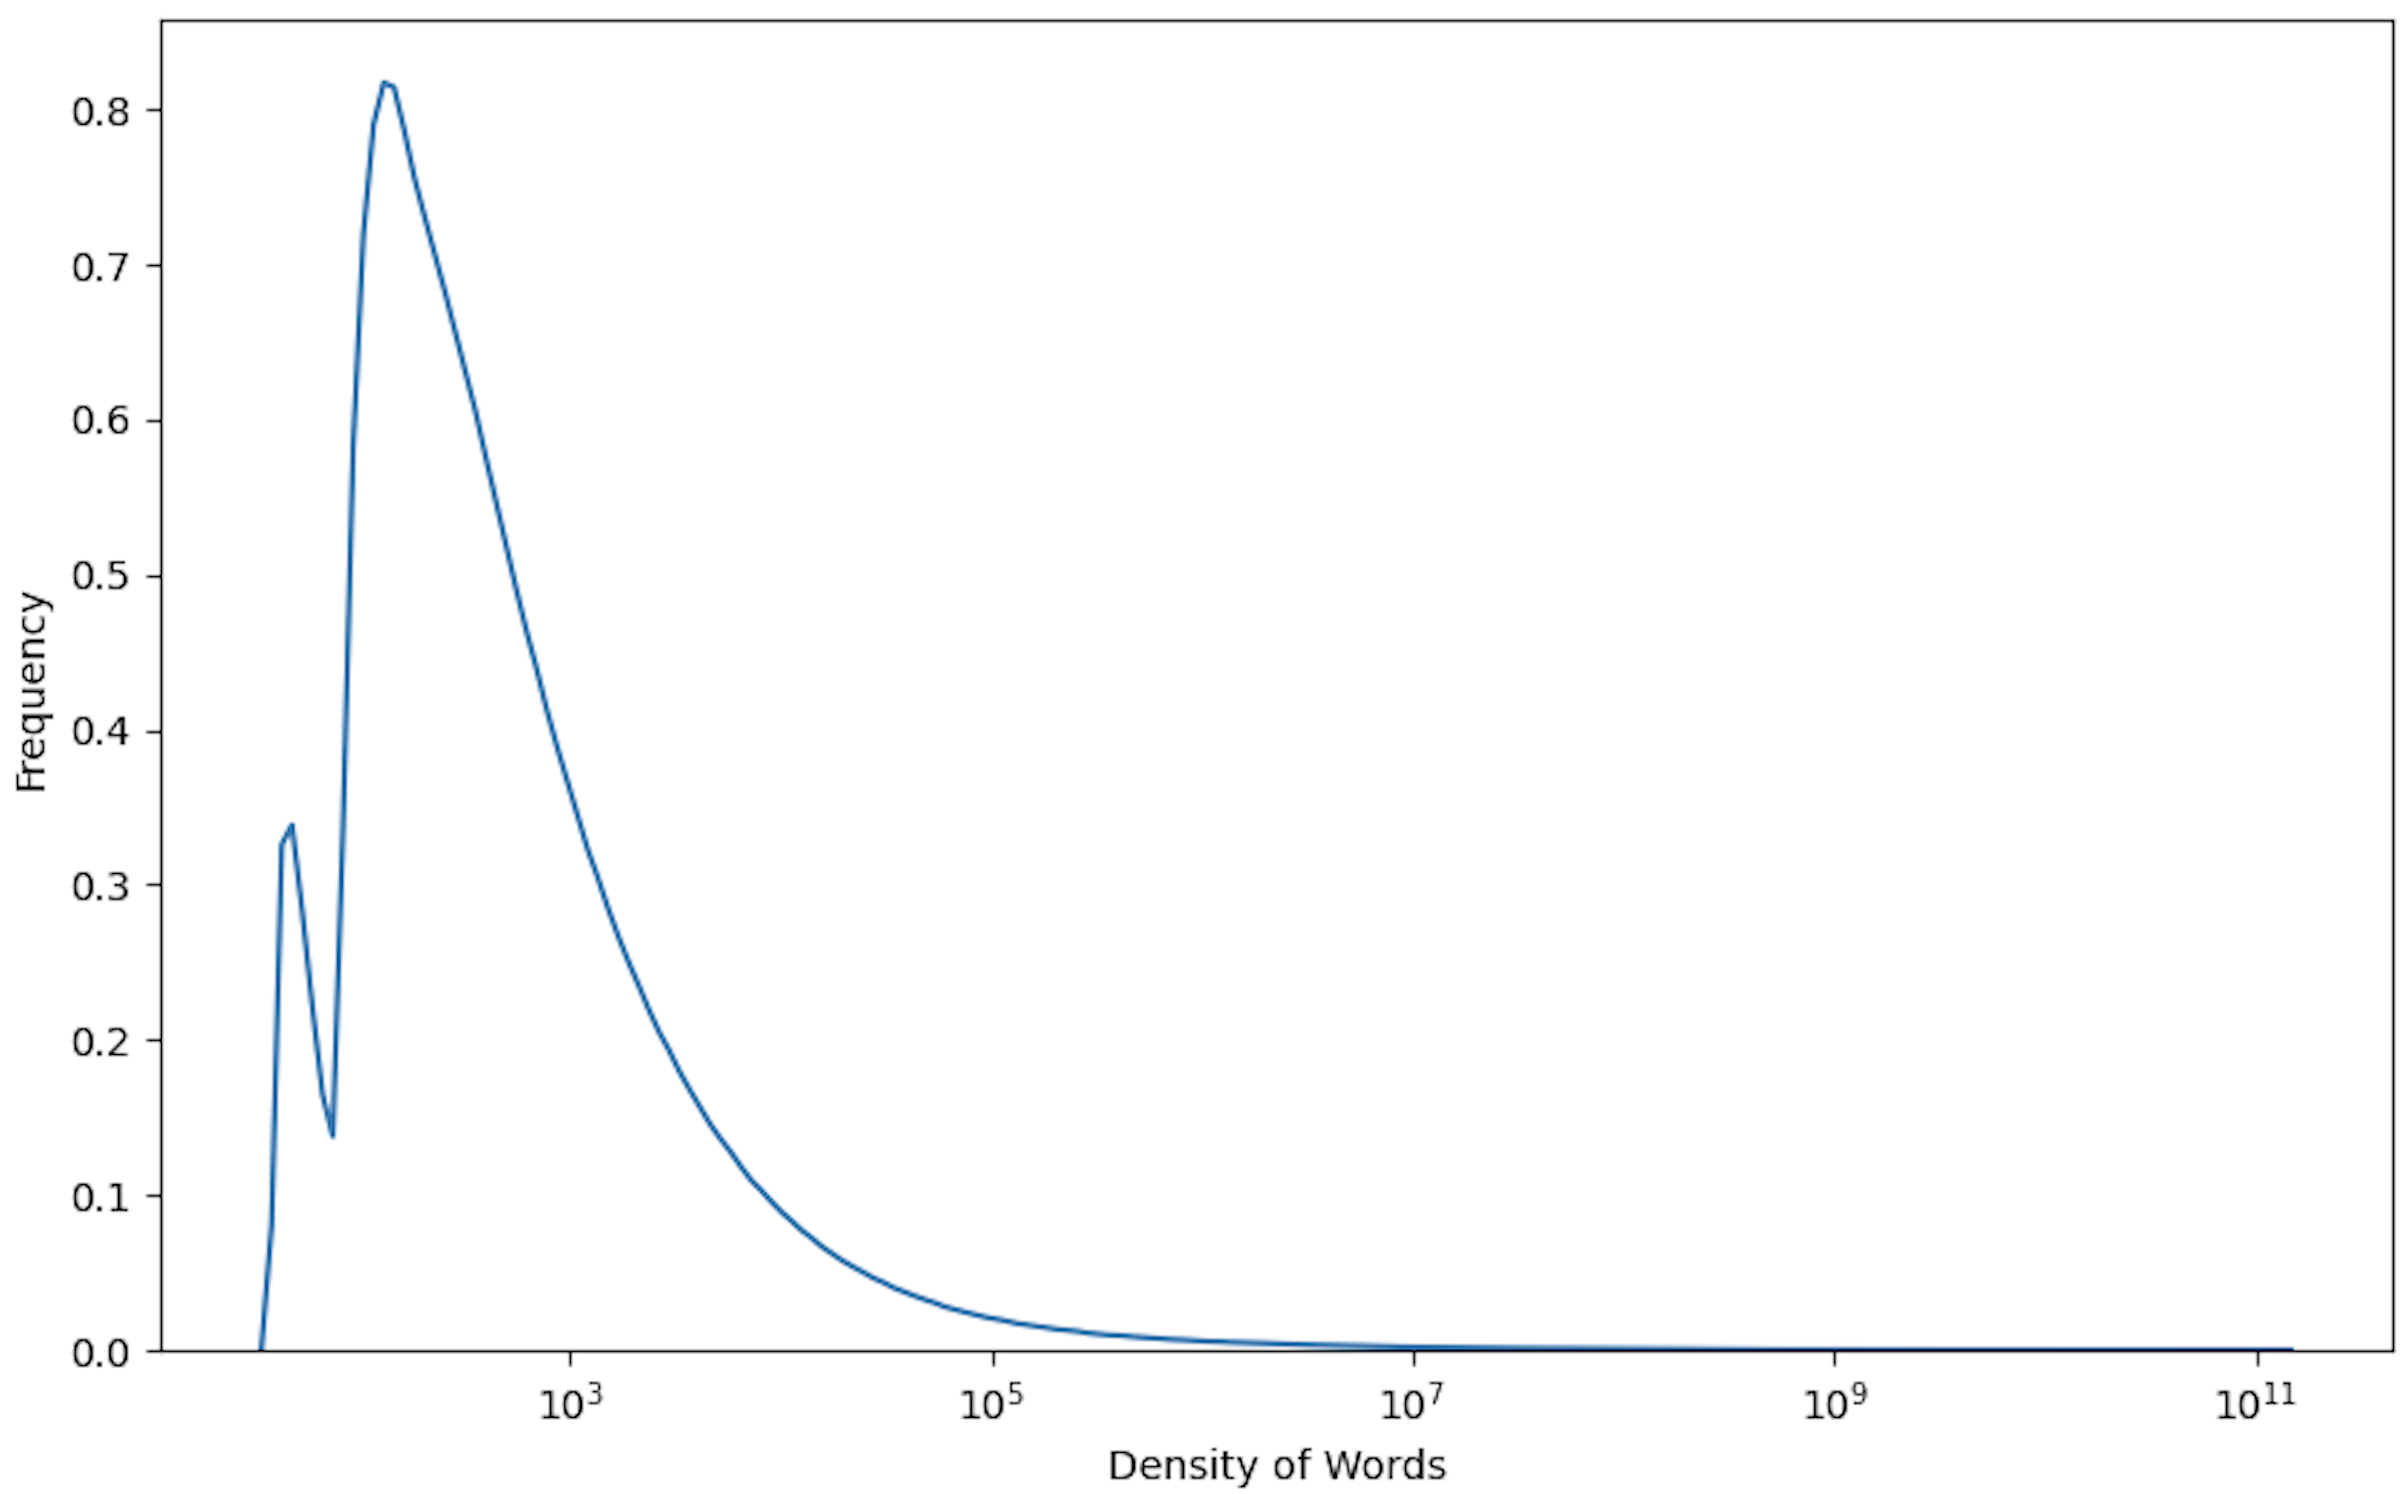
\includegraphics[width=0.7\textwidth]{KDE_freq.png}
    \caption{Kernel density estimate of frequency of the words}
    \label{fig:word_freq}
\end{figure}

Figure \ref{fig:word_freq} presents a kernel density estimate (KDE) of word frequencies, showing the distribution of word occurrence densities on a logarithmic scale. The x-axis represents the density of words (frequency counts), while the y-axis shows the estimated probability density. The words are highly left skewed, a typical pattern in natural language data. Most words have relatively low frequencies, with a sharp peak around $10^3$, indicating that a large portion of the vocabulary appears infrequently. As the frequency increases, the density rapidly declines, forming a long right tail that reflects a small number of words occurring extremely often. This distribution aligns with Zipf’s Law, which states that a few words dominate language usage while the rest of the words are rare. 

\section{Company Information} \label{sec:company_info}
This section presents details about the company names used in the regression in Section \ref{company_name} and their financial data in Section \ref{company_fin}. The company names will be utilized in the deep learning model, while the financial data will be employed in the panel regression to evaluate the effect of the fluency score.
\subsection{Company Name} \label{company_name}
The company name list is sourced from Compustat and includes global firms that have existed for more than three years. This threshold ensures a sufficient number of observations for robust and reliable analysis. The trained model assigns a fluency score to each name in this list.

After applying these selection criteria, the dataset consists of 12,057 companies. To standardize the names, legal suffixes such as ``Corp'', ``LLC'' and ``Inc'' are removed. Additionally, all special characters, numbers, punctuation marks, and single-letter entries are excluded to maintain consistency and improve data quality. Examples of the cleaned company names are given in Figure \ref{fig:company_name}.

\begin{figure}[h!]
    \centering
    
\includegraphics[width=0.8\textwidth]{company_name.png}
    \caption{Examples of processed company names}
    \label{fig:company_name}
\end{figure}

\subsection{Company Financials} \label{company_fin}
To comprehensively assess the effect of company name fluency on firm outcomes, a set of control variables from the Compustat database is incorporated into the regression model. These control variables help isolate the unique contribution of the fluency score by accounting for other firm-specific factors that could influence valuation, liquidity, or performance. The dataset used for the regressions is structured on a quarterly basis, covering a period from January 1980 to December 2024.

To maintain data integrity and ensure reliable estimation, the panel regression omits any dependent observations with missing values and keep companies where all the quarters have data. This approach prevents biases that could arise from incomplete data and supports the robustness of the regression analysis. Valuation, liquidity and performance respectively have 15,274, 5,574 and 9,850 unique companies respectively, in the dataset. Table \ref{tab:summary_performance} provides the summary statistics of the variables used in panel regressions. 

\begin{table}[h]
\centering
\caption{Summary statistics for financial variables}
\label{tab:summary_performance}
\begin{tabular}{llcccc}
\toprule
\textbf{Category} & \textbf{Variable} & \textbf{Observations} & \textbf{Mean} & \textbf{Min} & \textbf{Max} \\
\midrule
\multirow{4}{*}{Valuation} 
    & \texttt{Market-to-Book Ratio}      & 631,274 & 7430.038    & -1.290e09   & 1.370e09  \\
    & \texttt{Sales} &  627,924 & 25.670     & -362.437   & 1.440e70  \\
    & \texttt{Profitability}           & 573,370  & -0.018     & -23500   & 1751  \\
    & \texttt{Leverage}      & 624,525 & 0.245     & -0.093   &  5010 \\
\bottomrule
\multirow{6}{*}{Liquidity} 
    & \texttt{Liquidity Measure}&  243,858  & 19.520     & 7.699   & 29.332  \\
    & \texttt{Size} &  201,713 & 6.921     & -8.511   & 15.074  \\
    & \texttt{Profitability} & 168,394 & 0.062    & -12.095   & 5.708  \\
    & \texttt{Valuation}      & 175,869  & 2027.464     & -1.700e07   & 5.150e07 \\
    & \texttt{Price} & 204,519 & 0.218 & 2.907e-4    & 10000\\
    & \texttt{Volatility} & 243,772 & 0.027 & 0    & 5.007 \\
\bottomrule
\multirow{3}{*}{Performance} 
    & \texttt{Gross return on stock}      & 436,340 & 0.012     & -0.863   & 8.335  \\
    & \texttt{Size} & 416,508  & 5.980     &  -8.512   & 15.074  \\
    & \texttt{Profitability}  & 368,596 & 0.075     & -21.476    & 9.930  \\
    & \texttt{Price}  & 426,152 & 0.252     & 2.013e-4    &  10000 \\
\bottomrule
\end{tabular}
\end{table}



\chapter{Methodology} \label{sec:neural_network}
The chapter is divided into three parts. The first part consists of features of the words used to fit the fluency score. The second part is the deep learning model and its parameters used to predict the fluency score for the company names. The third, and last, part presents the evaluation of the fluency score by measuring the effects on valuation, liquidity, and performance to estimate the effects.

\section{Features}
Words have different features which can be used as input for a deep learning model to predict the fluency score. The next section provides a detailed explanation of the features, including the rationale behind their selection and how they are computed.

\subsection{Englishness Score}
\citeA{englishness_score} coined the term \textit{Englishness score}, which measures how `English' a word is using conditional bi- and trigram probabilities. A word is more English if it consists of more commonly found bi- and trigrams in the English language, in this case the lexicon dataset. An example of this feature is that ``th'' will have a higher Englishness score if the third letter is ``e'' compared to the third letter being ``l''. This is because ``the'' is more frequently seen in the text compared to ``thl''.

A \textit{n}-letter string can be denoted as: \#$L_1$, $L_2$, $L_3$, ..., $L_k$, ..., $L_n$\# where \# denotes the space (spaces only occur at beginning or the end of a string) and $L_i$ denotes the letter in the $\textit{i }^{th}$ position in the string. The Englishness score (E) is defined as the total conditional probability of the \textit{n}-letter string using bi- and trigrams, 
\begin{align}
E &= P(\# L_1, L_2, L_3, \ldots, L_k, \ldots, L_n \#) \nonumber \\
  &= P(\#) \cdot P(L_1 \mid \#) \cdot P(L_2 \mid \# L_1) \cdot P(L_3 \mid L_1 L_2), \ldots , P(L_k \mid L_{k-2} L_{k-1}), \ldots, P(\# \mid L_{n-1}, L_n)
\label{eq:equation1}
\end{align}
The conditional probability is estimated as the following, 
\begin{align}
P(L_k \mid L_{k-2} L_{k-1}) \approx \frac{F(L_{k-2}L_{k-1}L_k)}{F(L_{k-2}L_{k-1})}
\label{eq:equation2}
\end{align}

\noindent where F denotes the number of occurrences of the bi- or trigrams in the English language. The words in the lexicon list are used to count the number of occurrences of each possible bi- or trigram. By substituting Equation \ref{eq:equation2} into Equation \ref{eq:equation1}, approximation of E can be depicted as, 
\begin{align}
    E \approx \frac{F(\#)}{F(ALL)} \cdot \frac{F(\#L_1)}{F(\#)} \cdot \frac{F(\#L_1L_2)}{F(\# L_1)} \cdot \frac{F(L_1 L_2 L_3)}{F(L_1 L_2)} , \ldots, \frac{F(L_{k-2}L_{k-1}L_{k})}{F(L_{k-2}L_{k-1})} , \ldots, \frac{F(L_{n-1}L_n\#)}{F(L_{n-1}L_n)}
\label{eq:equation3}
\end{align}
in which $F(ALL)$ is the count of all the characters. The terms $F(\#)$ and $F(\#L_1)$ can be cancelled out. The term $1/F(ALL)$ is ignored as it appears in all strings and thus does not contribute to the relative Englishness score. Thus the Equation \ref{eq:equation3} can be simplified to:
\begin{align}
    E' = {F(\#L_1L_2)}\cdot \frac{F(L_1 L_2 L_3)}{F(L_1 L_2)} , \ldots, \frac{F(L_{k-2}L_{k-1}L_{k})}{F(L_{k-2}L_{k-1})} , \ldots, \frac{F(L_{n-1}L_n\#)}{F(L_{n-1}L_n)}
\label{eq:equation4}
\end{align}
As the Equation \ref{eq:equation4} will yield very small values for $E'$, hence it is better to use negative logarithm of the product which is indicated by $E''$.
\begin{align}
    E'' = -\left[logF(\#L_1L_2) + log\frac{F(L_1 L_2 L_3)}{F(L_1 L_2)} + \ldots + log \frac{F(L_{k-2}L_{k-1}L_{k})}{F(L_{k-2}L_{k-1})} + \ldots + log \frac{F(L_{n-1}L_n\#)}{F(L_{n-1}L_n)}\right]
\label{eq:equation5}
\end{align}
The Englishness score calculated from Equation \ref{eq:equation5} is likely to be influenced by word length, as longer words are generally less frequent and thus may appear less fluent or familiar. To address this, \citeA{englishness_score} adjusted for length by dividing each word’s $E''$ score by the word's length. In contrast, \citeA{fleuncy2_main} proposed a more statistically robust method by regressing the $E''$ score on word length and using the resulting residuals as the adjusted Englishness scores. This approach isolates the component of fluency that is independent of word length, allowing for a cleaner interpretation of linguistic familiarity. Following this rationale, the study adopts the regression-based method to control for word length effects.

For names consisting of multiple words, the overall Englishness score is computed as the sum of the individual scores of each constituent word. Similarly, the total length of the name is defined as the sum of the lengths of its component words. In some cases, a word or name may include bi- or trigrams that are not present in the lexicon, rendering the calculation in Equation \ref{eq:equation5} infeasible. To overcome this issue, a small conditional probability of 0.1\% is assigned when a bigram is missing, under the assumption that its associated trigrams are also absent. If the bigram exists but the corresponding trigram is not found, an ad hoc estimate of the conditional probability is used, calculated as the inverse of the total number of bigrams \cite{bigram_ref}. Examples of the Englishness score are given in Figure \ref{fig:englishness_score}. 

\begin{figure}[h!]
    \centering
    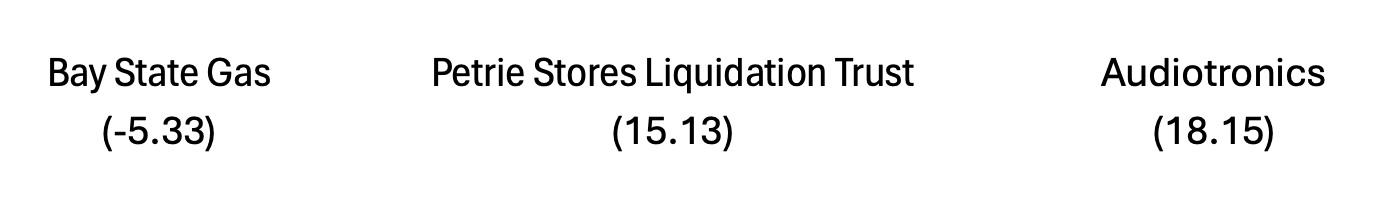
\includegraphics[width=0.7\textwidth]{englishness.png}
    \caption{Examples of Englishness scores}
    \label{fig:englishness_score}
\end{figure}

\subsection{Word Length}

\citeA{word_length1} has found through experiments that memory span decreases as the word length increases. Shorter spoken words are recalled more accurately compared to longer spoken words hence, having a short word in the company's name can help people recall the name easier. A study by \citeA{word_length2} investigates the factors that affect the readability of books and finds out that sentence length and complexity of the sentences are the main factors affecting the readability. Hence, having shorter sentences with simpler structures can help improve the readability. In their work, \citeA{kincaid1975readability} developed formulas such as the Automated Readability Index (ARI), Fog Count, and Flesch Reading Ease to assess the readability of documents. One of the key components in these formulas is the average number of words per sentence. However, since the focus of the current research is on company names rather than entire documents, this characteristic will be adapted to measure average word length instead, as it better reflects the structure and complexity of names rather than using full sentences. Examples of the word length features are shown in Figure \ref{fig:word_length}.

\begin{figure}[h!]
    \centering
    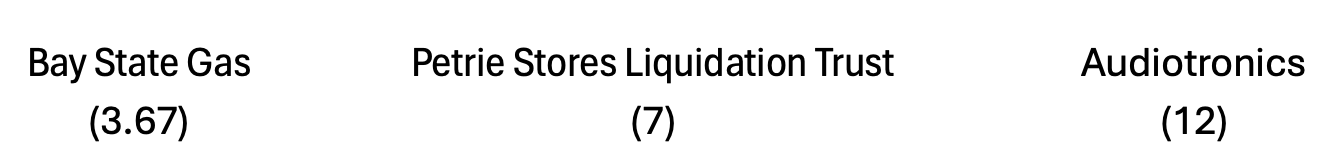
\includegraphics[width=0.7\textwidth]{word_length.png}
    \caption{Examples of word length feature}
    \label{fig:word_length}
\end{figure}

\subsection{Syllable}
Another feature proposed by \citeA{kincaid1975readability} is the average amount of the syllables per word, but this can be correlated to the average word length. In this research, both features are retained, as they offer complementary insights into the fluency and complexity of words. While longer words generally tend to have more syllables (e.g., ``international'' has 6 syllables and 13 letters), this correlation does not always hold. For example, ``queue'' has only one syllable but five letters, while ``idea'' has three syllables but only four letters. These exceptions highlight the value of considering both features separately to better capture nuances in name fluency and readability. Examples of the syllable features are given in Figure \ref{fig:syllables}.

\begin{figure}[h!]
    \centering
    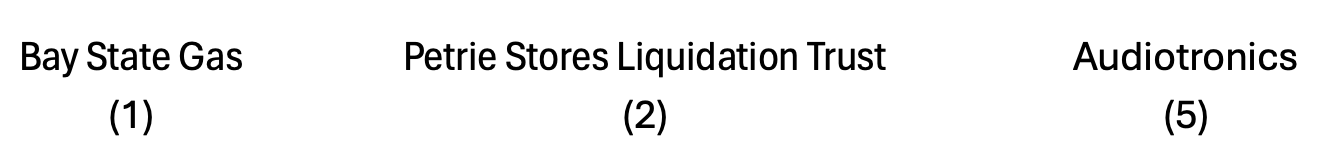
\includegraphics[width=0.7\textwidth]{syllabus.png}
    \caption{Examples of syllable features}
    \label{fig:syllables}
\end{figure}

\subsection{Alphabetical Order}
Investors are often impacted by alphabetical bias, wherein early alphabet stocks are traded more frequently than the later alphabet stocks \cite{alpha, AlphabeticBias}. Stocks with names that begin with earlier letters in the alphabet often experience higher trading volumes and greater liquidity. This phenomenon is attributed to limited investor attention and the use of heuristic processing, investors typically being unable to process all available information. As a result, stocks that are more readily visible, such as those appearing earlier in alphabetical lists, may attract disproportionate attention and generate a visibility bias in investment decisions. To identify potential ordering bias, one-hot encoding is applied on the first letter of each word. Specifically, the first variable is assigned a value of 1 if the word begins with a letter from the set \{a, b, c, d, e\}, capturing the primacy effect. The second variable is set to 1 if the initial letter falls within the range \{f,...,u\}, while the third variable is set to 1 if the first letter is among \{v, w, x, y, z\}. This encoding scheme allows us to isolate and analyse the influence of the alphabetical position, particularly the bias toward words appearing earlier in the alphabet. Examples of the alphabetical order features are shown in Figure \ref{fig:alpha}.

\begin{figure}[h!]
    \centering
    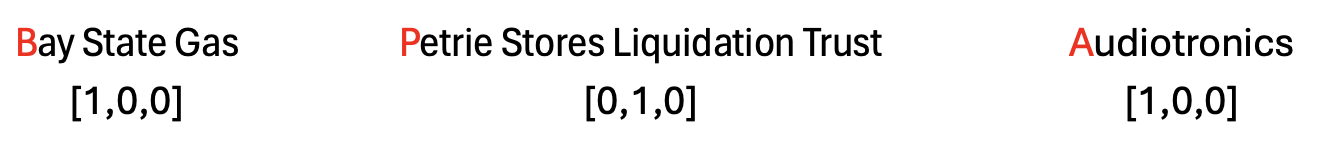
\includegraphics[width=0.7\textwidth]{alpha.png}
    \caption{Examples of alphabetical features}
    \label{fig:alpha}
\end{figure}

\subsection{Vowels and Consonants}
\citeA{sylla2_sound} demonstrate that the phonetic composition of a word can shape consumer perceptions and preferences, even when the word has no inherent meaning. Specific arrangements of vowels and consonants can subtly convey impressions related to size, strength, elegance, or other qualities. As a result, a vowel density of a word can be used to get insights in the  potential perceptual effects. Vowel density indirectly represents the consonants density as well, as they are linearly related to each other. In this study, vowels are defined as ``a'', ``e'', ``i'', ``o'', ``u'', and ``y''. Examples of the vowel features are given in Figure \ref{fig:vowel}.

\begin{figure}[h!]
    \centering
    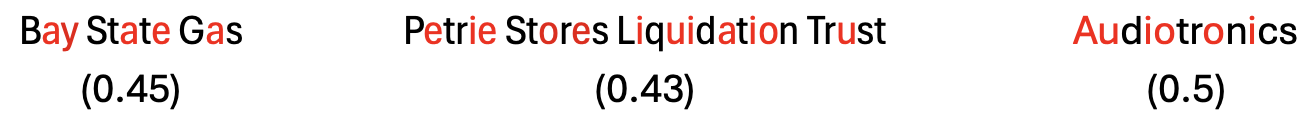
\includegraphics[width=0.7\textwidth]{vowel.png}
    \caption{Examples of vowel features}
    \label{fig:vowel}
\end{figure}

\subsection{Repetition}
\citeA{birds_repe} carried out a between-subjects experiment where participants evaluated the accuracy of various aphorisms. Some participants were instructed to disregard poetic elements and focus solely on content, while others received no such guidance. The study revealed the presence of the rhyme-as-reason effect, showing that rhyming aphorisms were perceived as more accurate than their non-rhyming counterparts. This is attributed to the enhanced processing fluency that rhyme provides. To approximate the influence of rhyme, we include a feature representing the frequency of the most common letter in a firm's name. This characteristic, especially when used alongside other phonetic or structural features, may help capture aspects of rhyme or repetition that contribute to the perceived fluency of a word. Examples of the repetition features are shown in Figure \ref{fig:rep}.

\begin{figure}[h!]
    \centering
    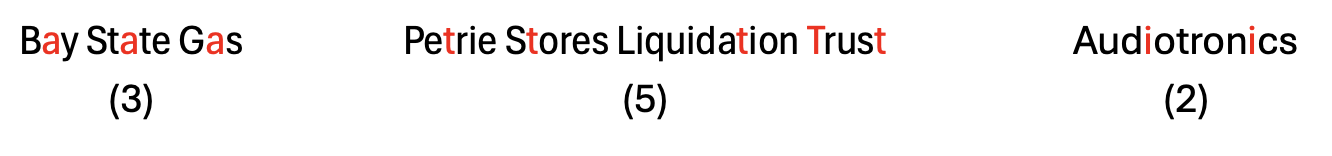
\includegraphics[width=0.7\textwidth]{repetition.png}
    \caption{Examples of repetition features}
    \label{fig:rep}
\end{figure}

\subsection{Spelling}
Another word feature is the spelling which stems from the dictionary feature of \citeA{fleuncy2_main}. If a word within a company name is flagged as misspelled by the spell-checker, the corresponding feature is assigned a value of 1, otherwise, it is assigned a value of 0. This results in a binary variable that indicates whether a firm name contains any spelling errors. Such errors can be interpreted as a form of disfluency. While the original dictionary score was derived using Microsoft’s spell-checker as part of an unsupervised method, this study employs the Enchant spell-checking library. Spell-checks are conducted using both American English and British English dictionaries, meaning a word will not be marked as misspelled if it is deemed correct in at least one of the two variants. Examples of the spelling features are given in Figure \ref{fig:spell}.

\begin{figure}[h!]
    \centering
    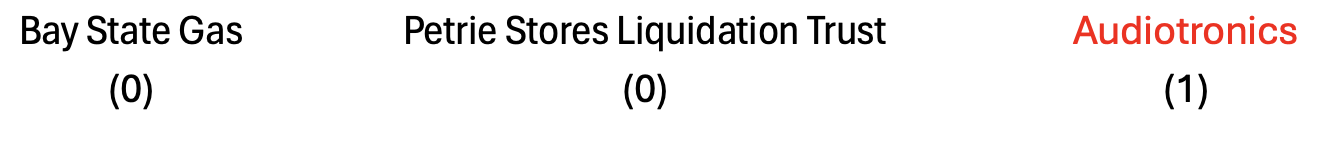
\includegraphics[width=0.7\textwidth]{spell.png}
    \caption{Examples of spelling features}
    \label{fig:spell}
\end{figure}

\subsection{Short Name}
\citeA{impor_name1} showed that short and snappy names are processed more quickly whereas longer names create a distinct identity in people's minds, making them well-suited for luxury brands by enhancing memorability and setting them apart. If a company name has less than 2 words then it is assigned a score of 1 else it is assigned 0. This results in a binary variable indicating whether a firm has a long or short name. Examples of the short name features are shown in Figure \ref{fig:rep}.

\begin{figure}[h!]
    \centering
    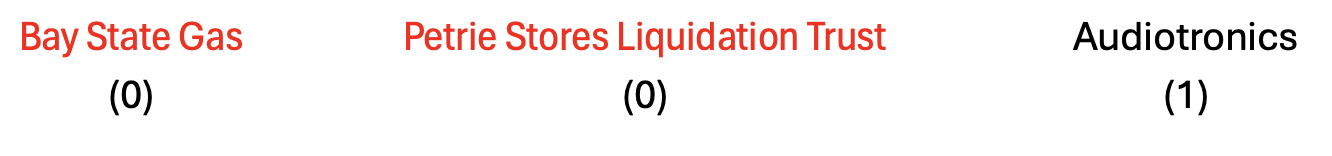
\includegraphics[width=0.7\textwidth]{short_name.png}
    \caption{Examples of short name features}
    \label{fig:short_name}
\end{figure}

\subsection{Pronunciation}
The last feature used in the deep learning model is the pronunciation of the words. Through experiments, \citeA{sound} show that easy pronunciation enhances the positive impact of connotation, while difficult-to-pronounce names diminish this effect. \citeA{sylla1} use experiments to show that participants lean towards names with fewer syllables and deem them as less risky and more trustworthy compared to difficult-to-pronounce names, due to heightened perceptions of novelty. This effect is consistent across contexts like food safety and entertainment, and is not driven by emotional responses but rather by how novel the stimuli seem. To capture the phonetic qualities of company names, a Soundex score is generated using the phonetics Python library (\url{https://pypi.org/project/phonetics/}). For each company name, the longest word is selected and converted into a four-character code reflecting its English pronunciation. This score enables identification of similarly sounding names, adding a phonetic dimension to the linguistic analysis. Examples of the pronunciation features are given in Figure \ref{fig:sound_name}.

\begin{figure}[h!]
    \centering
    
\includegraphics[width=0.7\textwidth]{sound.png}
    \caption{Examples of pronunciation features}
    \label{fig:sound_name}
\end{figure}



\section{Deep Learning Model} \label{deep_learning_model}
This section presents the deep learning model designed to predict the fluency score using company name features. It provides a detailed description of the model architecture and concludes with an evaluation of its performance relative to benchmark models.

\subsection{Model Architecture}
The model is trained to learn the relationship between standardized linguistic features of English words and their corresponding frequency values. Here, frequency acts as a proxy for processing fluency, which reflects how easily a word is recognized and understood. The purpose of this training is to enable the model to predict a word’s fluency based on its structural characteristics, such as word length, phonetic composition, or character-level n-grams.

Once trained, the model is used to estimate fluency scores for company names. This application is based on the assumption that the statistical features influencing fluency in regular English words are similarly applicable to company names. Although company names may vary in format or creativity, they are ultimately constructed from the same fundamental elements: letters from the English alphabet. These names are subject to the same underlying distributional properties that govern word formation in the language. Given this common linguistic foundation, names containing unusual letter patterns or uncommon n-grams are likely to be perceived as less fluent or less English-like, similar to how rare or irregular words are processed. This assumption supports the generalizability of the model from a lexicon of common words to a broader set of company names.

The implementation of the deep learning model involves optimizing a loss function that measures the discrepancy between the predicted and actual values. For regression tasks, one of the most commonly used loss functions is the Mean Squared Error (MSE), defined as:

\begin{align}
    \text{MSE} = \frac{1}{N} \sum_{i=1}^N (y_i - \hat{y_i})^2
\end{align}

\noindent where N denotes the total number of observations, company names in this case, $y_i$ is the actual fluency score of the $i^{th}$ observation, and $\hat{y_i}$ is the predicted score. However, a known drawback of the MSE is its sensitivity to outliers due to the squaring of the error term. In this context, fluency is proxied by word frequency, and word frequencies tend to follow a power-law distribution, where a few words are extremely common while most are rare. This is a well-documented empirical regularity and is consistent with Zipf’s Law \cite{zipf}, which shows that the frequency of a word is inversely proportional to its rank in a frequency list.

Given this heavily skewed distribution, using MSE could lead the model to disproportionately prioritize high-frequency words, thereby introducing a bias. To address this concern, the Mean Absolute Error (MAE) can be used:

\begin{align}
    \text{MAE} = \frac{1}{N} \sum_{i=1}^N \left| y_i - \hat{y}_i \right|
\end{align}

\noindent Unlike MSE, MAE measures the average magnitude of prediction errors without squaring them, making it less sensitive to outliers. It provides a more robust measure when dealing with data that exhibit power-law behaviour by penalizing the errors linearly instead of quadratically. However, a drawback of MAE is that it treats all errors equally, regardless of their size, and can therefore under-penalize large deviations. In the present context, fluency follows a power-law distribution, where a small number of words occur extremely frequently while most are rare. This imbalance means that large prediction errors for common words can have the same influence on the loss as small errors for rare words.

To address this concern, the Huber function is employed as both the loss and the evaluation function:

\begin{align}
    \text{Huber}_{\delta} = \frac{1}{N} \sum_{i=1}^N 
    \begin{cases}
        \frac{1}{2}(y_i - \hat{y_i})^2 & \text{for } |y_i - \hat{y_i}| \leq \delta, \\
        \delta \cdot |y_i - \hat{y_i}| - \frac{1}{2} \delta^2 & \text{otherwise},
    \end{cases}
\end{align}

\noindent While MSE penalizes large errors heavily and MAE treats all errors equally, the Huber loss offers a compromise that combines the advantages of both. For small residuals, it behaves like MSE, applying a quadratic penalty that encourages precise predictions, while for large residuals beyond a specified threshold $\delta$, it switches to a linear penalty similar to MAE, thereby reducing sensitivity to outliers. This makes it particularly suitable for predicting fluency scores, which are based on word frequencies that follow a power-law distribution. In such data, a small set of extremely common words can produce large prediction errors, while the vast majority of rare words yield smaller errors. The Huber loss can mitigate the disproportionate influence of these outliers without under-penalizing smaller deviations, ensuring a balanced optimization process that preserves accuracy across the frequency spectrum.

The deep learning model also consists of several hyperparameters that need to be tuned. To achieve this, the frequency list is divided into three subsets: 70\% of the data is allocated for training during hyperparameter tuning, while the remaining 30\% is evenly split—15\% for validation during tuning and 15\% for testing the final tuned model. During hyperparameter tuning, a Hyperband search is conducted using Keras Tuner with a maximum of 20 epochs per trial and a reduction factor of 2. The reduction factor determines how aggressively the search narrows down poorly performing configurations. After each round, only half of the trials with the lowest performance continue to the next stage, allowing the tuner to allocate more resources to promising hyperparameter combinations while quickly eliminating suboptimal ones. This approach results in an efficient exploration of the hyperparameter search space. The objective is to minimize the validation loss. To enhance training stability and convergence, early stopping is applied with a patience of 5 epochs using EarlyStopping (\url{https://keras.io/api/callbacks/early_stopping/}). This means that if the validation performance does not improve for 5 consecutive epochs, training stops and the model reverts to the weights corresponding to the best observed validation score. To further enhance training stability and convergence, a learning rate scheduler is applied using ReduceLROnPlateau (\url{https://keras.io/api/callbacks/reduce_lr_on_plateau/}). This mechanism monitors the validation loss and reduces the learning rate by a factor of 0.5 if no improvement is observed for 3 consecutive epochs, with a lower bound of $1 \times 10^6$. By decreasing the learning rate when progress stalls, the model can take smaller, more precise steps toward the loss minimum, helping to achieve smoother convergence and improved generalization.

Each model is trained using mini-batches of 1,000 observations. The number of hidden layers is treated as a tunable parameter and varied across the set \{1, 2, 3, 4, 5, 6\}. Each hidden layer in the model uses either the ReLU activation function \cite{relu}, the Tanh activation function \cite{tanh} or the Sigmoid activation function\cite{sigmoid}, depending on which yields better performance during tuning. The Tanh function maps inputs to the range [-1, 1], enabling centred activations that can improve training dynamics, while the Sigmoid function maps inputs to [0, 1], making it suitable for probabilistic interpretations and smooth non-linear transformations. The ReLU activation function outputs the input directly if it is positive, and zero otherwise, introducing non-linearity while avoiding vanishing gradients.

The output layer uses a linear activation function, appropriate for regression tasks. To determine the optimal network architecture, the number of nodes per hidden layer is searched over the set \{4, 8, 16, 32\}. To prevent overfitting, L1 and L2 regularization is applied to the weights of each node and are tuned using values \{0.0, 0.01 ,0.001\}. During hyperparameter tuning, each hidden layer can optionally include batch normalization and dropout. Batch normalization standardizes the inputs to a layer, maintaining a mean of zero and a standard deviation of one, which stabilizes training and allows for higher learning rates. Dropout, when selected, randomly deactivates a fraction of neurons in the layer during training, with the dropout rate chosen from a set of hyperparameters \{0.1, 0.2, or 0.3\}. This reduces overfitting, and encourages the network to learn more robust representations. Additionally, the model is compiled using the Adam optimizer \cite{adam} with the initial learning rate selected as a hyperparameter from the set \{0.01, 0.001 ,0.0001\}. Lastly, the Huber loss function has the $\delta = 1$. The entire framework is implemented in Python using the Keras deep learning library (\url{https://keras.io/}).

\subsection{Model Training and Benchmarking}
Once the model has been trained and tuned using 85\% of the observations from the frequency list, the remaining 15\% is reserved to evaluate its performance on out-of-sample data. This is a crucial step as it tests the model’s ability to generalize beyond the data it was trained on, ensuring that it does not just memorize the training data. By evaluating on unseen data, the model's robustness and predictive power is gauged. To assess its performance, five benchmark methods are used to compare how well the model performs in predicting fluency scores on the out-of-sample data: 

\begin{itemize}
    \item Uniform distribution: This benchmark involves generating random fluency scores for the test observations, drawn from a uniform distribution that spans the minimum and maximum fluency scores observed in the training data. The uniform distribution assumes that every score within the range is equally likely to be assigned to a test observation. By using this benchmark, the goal is to evaluate how the model compares against a random, equally distributed assignment of fluency scores.
    \item Normal distribution: In this approach, fluency scores for the test observations are drawn from a normal distribution, where the mean and standard deviation match those of the fluency scores in the training set. This assumes that the test data follows a similar statistical pattern as the training data. This benchmark tests how well the model performs compared to a random assignment of fluency scores that aligns with the statistical properties of the training set.
    \item Training distribution: Fluency scores are sampled with replacement from the training data and assigned to the test observations. Essentially, this method creates multiple random samples from the training data, reflecting the variability inherent in the dataset. This benchmark helps assess how the model compares against random assignments of fluency scores sampled from the same distribution as the training set.
    \item Zipf's distribution: In this benchmark, fluency scores for test observations are drawn from a Zipf's distribution, a type of power-law distribution where lower scores are significantly more probable than higher ones. This reflects the idea that, in many natural language and social phenomena, a small number of items occur very frequently while the rest are rare. By using this distribution, the benchmark evaluates how the model performs compared to a skewed, heavy-tailed distribution, which introduces a bias toward lower fluency scores and mirrors real-world frequency imbalances.
    \item Ordinary Least Squares regression: This benchmark involves fitting an OLS regression model on the training data to predict fluency scores for the test observations. The OLS regression serves as a simple linear approach, and by using it, we can compare how well the model performs relative to a traditional statistical method.
\end{itemize}

\noindent Table \ref{tab:intrinsic} gives an overview of the out-of-sample performance, measured by Huber Loss function, compared to the benchmark models.
\begin{table}[h!]
\centering
\renewcommand{\arraystretch}{1.5} % Increases row height by 1.5x
\caption{Performance metrics for different sampling methods}
\begin{tabular}{lcccccc}
\hline
\textbf{Metric} & \textbf{Uniform} & \textbf{Normal} & \textbf{Training} & \textbf{Zipf} & \textbf{OLS} & \textbf{Neural} \\
\hline
Huber Loss & $6.299 \times 10^{10}$ & $4.985 \times 10^{7}$ & $3.973 \times 10^{5}$ & $1.224 \times 10^{6}$ & $6.333 \times 10^{5}$ & $2.068 \times 10^{5}$ \\
\hline
\label{tab:intrinsic}
\end{tabular}
\end{table}

\noindent The Uniform distribution benchmark, which samples uniformly across the range of training target values, yields the highest Huber loss of $6.299 \times 10^{10}$. This indicates its poor fit due to the lack of any informed structure in prediction. The Normal distribution benchmark, which samples based on the training set's mean and standard deviation, performs considerably better, with a Huber loss of $4.985 \times 10^{7}$, serving as a naïve baseline informed by the global distribution. Sampling directly from the training distribution, randomly drawing values from the training target itself, produces the lowest errors among the non-parametric benchmarks, with a Huber loss of $3.973 \times 10^{5}$. This shows that this method most closely resembles the true data-generating process. The Zipf distribution, known for its heavy-tailed structure, leads to a moderate performance, with  a Huber loss of $1.224 \times 10^{6}$, reflecting its mismatch with the actual data distribution. Finally, the Ordinary Least Squares (OLS) regression model achieves a Huber loss of $6.333 \times 10^{5}$. While not as accurate as direct training distribution sampling, OLS outperforms all purely random benchmarks and offers interpretable parameter estimates, making it a valuable baseline for comparison. The neural network model, which leverages the full feature set, achieves the lowest Huber loss overall at $2.068 \times 10^{5}$, highlighting its ability to capture complex relationships and improve the prediction of firm name fluency.

Overall, the intrinsic results demonstrate that the neural network model substantially outperforms all benchmark methods. By leveraging the features of the words and capturing complex non-linear relationships, the neural network achieves the lowest Huber loss. This highlights its advantage in modelling intricate patterns in the data, providing a more precise and robust alternative to simpler or purely random baseline approaches.
After the \textit{intrinsic} evaluation, the model is trained again using all the data from the frequency list. This step ensures that the final model makes full use of all available information. By learning from all the observations, the model can improve its predictions and provide more accurate fluency scores for company names.

\section{Evaluation of Fluency Scoring} \label{evaluation_fluency_score}
Additional to the intrinsic evaluation, an extrinsic evaluation takes place which examines how well the fluency score explains the stock characteristics. This is done via panel regressions with fixed effects where quarterly observation of stock characteristics are regressed on the fluency score and lagged control variables. A Difference-in-Difference (DiD) analysis is conducted to examine the immediate effects of a name change, followed by a cross-sectional regression to assess the long-term impact of company name fluency. The evaluation of fluency score is done via various aspects like valuation, liquidity, and performance.

\subsection{Valuation}
The market-to-book ratio is a key financial metric that reflects how the market values a company. The book value of a company is derived from its balance sheet and is calculated as the total assets minus the total liabilities. This figure represents the company’s net worth in the event of a full liquidation. On the other hand, the market value is determined by the current stock price multiplied by the number of outstanding shares, indicating how much investors are willing to pay for the company’s equity. Since investors tend to be forward-looking, the market value may differ from the book value. The market-to-book ratio is calculated by dividing the market value by the book value. This ratio reveals how much investors are willing to pay for every dollar of net assets, offering insight into investor perception and confidence in the company’s future prospects. A low market-to-book ratio could suggest that the company is undervalued, possibly presenting a buying opportunity, while a high ratio might indicate that the company is overvalued, potentially signalling risk.

Given that the valuation of a company is a crucial element for investors, understanding the factors that influence this valuation becomes important. One factor that may play a role in company valuation is the fluency of the firm’s name. To explore this, a fixed-effect panel regression analysis is conducted to examine the potential impact of firm name fluency on its market valuation. The fixed-effects regression model is as follows:
\begin{align}
    log \left[MB_{i,q}\right] = \beta_1log\left[F_{i,q}\right] + {\beta_2}C_{i,q-1} + \delta_s(i) + {\beta_3}log\left[F_{i,q}\right] \times \delta_s(i) + \gamma_q + \alpha_i + \epsilon_{i,q}
\end{align}
\noindent where $MB_{i,q}$ is the market-to-book ratio of company $i$ in quarter $q$. As shown in Table \ref{tab:summary_performance}, $MB_{i,q}$ has a large range from $-1.290e09$ to $-1.370e09$ with a mean of 7430, indicating the presence of extreme outliers. Applying logarithmic transformation to $MB_{i,q}$ ensure a more symmetric distribution and mitigates the influence of the outliers. $F_{i,q}$ is the predicted fluency score of company $i$ at quarter $q$, which is also log-transformed to facilitate clearer interpretation of results. $C_{i,q-1}$ is a vector containing control variables of company $i$ in quarter $q-1$ and $\delta_s(i)$ is the dummy variable for sector in which company $i$ operates in. Interaction term $log\left[F_{i,q}\right] \times \delta_s(i)$ allows the fluency $F_{i,q}$ on $MB_{i,q}$ to vary by sector. Including both the overall fluency slope and sector-specific slopes allows the fixed-effect regression to capture a general, baseline effect of fluency across all industries while also accounting for variations in its impact between sectors. This approach improves precision and enables sector-level comparisons. The $\gamma_q$ and $\alpha_i$ is the fixed effects for the four quarters and the company $i$ respectively. Each company’s valuation is controlled with the following variables:

\begin{itemize}
    \item Sales defined by \textit{sales/market capitalisation};
    \item Profitability defined by \textit{gross profit/total assets};
    \item Leverage defined by \textit{total debt/total assets}.
\end{itemize}

These control variables were also employed by \citeA{fleuncy2_main} in their analysis of the impact of company name fluency on firm valuation, and were originally introduced by \citeA{valuation1} in a study investigating the effects of valuation discounts in takeover scenarios. \citeA{fleuncy2_main} adds the Englishness score, the word length score and spell check score to create a fluency score whereas the methodology in this paper combines various word features to create a comprehensive fluency score that reflects how an investor processes the company name. 

To estimate the average causal effect of a company name change on market valuation, a Difference-in-Difference (DiD) analysis is employed \cite{card}. This method compares the change in market-to-book ratio for firms that experienced a name change (treatment group) with the change for firms that did not (control group), before and after the event. The indicator variable $\text{Treated}_i$ equals 1 for firms that underwent a name change, and 0 otherwise. The variable $\text{Post}_{i,q}$ equals 1 for quarters after the name change for treated firms, and 0 otherwise. The interaction term $\text{Treated}_i \times \text{Post}_{i,q}$ captures the DiD effect. The model is specified as,
\begin{align}
    \log\left[MB_{i,q}\right] = \beta_1 \left(\text{Treated}_i \times \text{Post}_{i,q}\right) 
    + \beta_2 C_{i,q-1} + \gamma_q + \alpha_i + \epsilon_{i,q}
\end{align}
where $C_{i,q-1}$ denotes the vector of control variables (sales, profitability, and leverage), $\gamma_q$ represents quarter fixed effects, $\alpha_i$ represents firm fixed effects, and $\epsilon_{i,q}$ is the error term. The coefficient $\beta_1$ captures the average change in the log market-to-book ratio attributable to the name change.

\begin{comment}
To understand the short terms effects of a company name change, an event study is conducted \cite{event_study1, event_study_2}. The analysis focuses on an event window spanning four quarters before and after the name change (i.e., from t $= -4$ to t = $= +4$), capturing any pre-event anticipation effects as well as the post-event market response over a one-year period. This allows for a balanced perspective on how investors react to changes in a firm’s name change within a relatively short time frame. The structure of event study is, 
\begin{align}
    log \left[MB_{i,q}\right] = \sum_{k=-4}^{4} \eta_k \cdot \text{REL}_{i,q}^{(k)} + {\beta_2}C_{i,q-1} +
               \gamma_q + \alpha_i + \epsilon_{i,q}
\end{align}
The control variable are same as the fixed-effect regression. $\text{REL}_{i,q}^{(k)}$ denotes dummy variables indicating the relative quarter $k$ from the event and $\eta_k$ capture the effect of the name change in each event-time quarter. $\gamma_q$ and $\alpha_i$
represent quarter and firm fixed effects respectively. 
\end{comment}

To further explore the effects of the fluency score, the dataset is collapsed into a cross-section format by averaging the values across time for each firm. This transformation enables the analysis of the relationship between firm valuation and company name fluency over a longer period of time. The cross-sectional regression model is as follows:
\begin{align}
    log \left[MB_{i}\right] = \beta_1 log\left[F_{i}\right] + {\beta_2} C_{i} + \delta{s(i)} + \epsilon_{i}
\end{align}

The control variables are same like in the fixed-effects regression and the term $\delta{s(i)}$ captures sector fixed effects to account for unobserved industry-level heterogeneity that may influence firm valuation. This specification helps isolate the effect of fluency from both firm-level fundamentals and sector-specific trends.

\subsection{Liquidity}
Liquidity, ease with which assets can be traded without causing significant price changes, is an important characteristic of stocks. It is an essential consideration for investors, as illiquid assets tend to experience higher price volatility and greater transaction costs. To quantify liquidity, this study employs the Amihud Illiquidity Measure \cite{amihud}, a widely used measure in financial research. It is defined as the average ratio of the absolute stock return to the corresponding traded volume. While the original formulation calculates this measure annually, it is adapted here to a quarterly frequency to align with the structure of the data:
\begin{align}
    ILLIQ_{i,q} = \frac{1}{D_{i,q}} \sum_{d=1}^{D_{i,q}} \frac{|R_{i,q}|}{V_{i,q}}
\end{align}

The $ILLIQ_{i,q}$ is the illiquidity measure of stock $i$ in quarter $q$. $D_{i,q}$ is the number of trading days in quarter $q$. $R_{i,q}$ and $V_{i,q}$ is the gross return and traded volume of stock 
$i$ in quarter $q$, respectively. A relatively high illiquidity measure indicates that a stock is less liquid, as it experiences larger price changes (high absolute returns) despite lower trading volumes. Conversely, a low illiquidity measure suggests higher liquidity, characterized by smaller price movements occurring alongside higher trading activity.

Panel regression with fixed effects is used to examine the effect of company name fluency on liquidity,

\begin{align}
    log\left[\frac{1}{ILLIQ_{i,q}}\right] = \beta_1log\left[F_{i,q}\right] + {\beta_2}C_{i,q-1} + \delta_s(i) + {\beta_3}log\left[F_{i,q}\right] \times \delta_s(i) + \gamma_q + \alpha_i + \epsilon_{i,q}
\label{liquidity}
\end{align}

The log inverse of the illiquidity measure is used as the dependent variable in Equation \ref{liquidity} to enhance the interpretability of the regression results. This transformation allows the left-hand side of the equation to be interpreted as a measure of liquidity. For clearer interpretation, the fluency score also has a logarithmic transformation. The $\delta_s(i)$ denotes a dummy variable for the sector in which company $i$ operates. The interaction term $log\left[F_{i,q}\right] \times \delta_s(i)$ allows the impact of fluency $F_{i,q}$ to vary across sectors, capturing heterogeneity in the model. As in the valuation regression, liquidity is modelled using firm name fluency, year-fixed effects, and a set of control variables. In this case, the following control variables are included:

\begin{itemize}
    \item Size defined by \textit{log(market capitalisation)};
    \item Profitability defined by \textit{gross profit/total assets};
    \item Valuation defined by \textit{market value/book value};
    \item Price defined by \textit{1/market price};
    \item Volatility defined by \textit{quarterly volatility}.
\end{itemize}

These control variables are derived from the study by \citeA{fleuncy2_main}, where they were employed to examine the influence of firm name fluency on the number of retail and institutional shareholders. The rationale behind this approach is the assumption that similar psychological factors may guide investor decisions regarding both stock ownership and trading behaviour.

As with valuation, a DiD approach is employed to examine changes in liquidity for firms undergoing a name change (treatment group) relative to those that did not (control group), comparing periods before and after the event. The model is specified as,
\begin{align}
    log\left[\frac{1}{ILLIQ_{i,q}}\right] = \beta_1 \left(\text{Treated}_i \times \text{Post}_{i,q}\right) 
    + \beta_2 C_{i,q-1} + \gamma_q + \alpha_i + \epsilon_{i,q}
\end{align}
where $C_{i,q-1}$ denotes the vector of control variables, $\gamma_q$ represents quarter fixed effects, $\alpha_i$ represents firm fixed effects. The interaction term $\text{Treated}_i \times \text{Post}_{i,q}$ captures the DiD effect. The coefficient $\beta_1$ captures the average change in the illiquidity measure due to the name change.
\begin{comment}
An event study is used to understand the short-term effect of change in company name. The study focuses on an event window spanning four quarters before and after the name change (i.e., from t $= -4$ to t = $= +4$), capturing any pre-event or post-event effect over a two-year period. Similar to valuation, the event study is structured as following, 
\begin{align}
    log\left[\frac{1}{ILLIQ_{i,q}}\right]  = \sum_{k=-4}^{4} \eta_k \cdot \text{REL}_{i,q}^{(k)} + {\beta_2}C_{i,q-1} +
               \gamma_q + \alpha_i + \epsilon_{i,q}
\end{align}
The control variable are same as the fixed-effect regression for liquidity. $\text{REL}_{i,q}^{(k)}$ is the dummy variable of the relative quarter $k$ from the event and $\eta_k$ capture the effect of the name change in each event-time quarter. $\gamma_q$ and $\alpha_i$
represent quarter and firm fixed effects respectively. 
\end{comment}
To further explore the effects of the fluency score, the dataset is converted into a cross-section format by averaging the values across time for each firm. This transformation allows us to understand the long-term effect between firm valuation and company name fluency. The cross-sectional regression model is:
\begin{align}
    log\left[\frac{1}{ILLIQ_{i}}\right] = \beta_1 log\left[F_{i}\right] + {\beta_2} C_{i} + \delta{s(i)} + \epsilon_{i}
\end{align}

The control variables remain consistent with those used in the fixed-effects regression. The term $\delta_{s(i)}$ now represents sector fixed effects, which control for unobserved industry-level heterogeneity that could influence firm liquidity. This specification allows for a clearer identification of the impact of fluency by accounting for both firm-specific fundamentals and sector-wide patterns.

\subsection{Performance}
Lastly, the influence of company name fluency is analysed in relation to stock performance, measured by realized quarterly gross returns. Stock performance is a key evaluation metric because it reflects how investors value a company and respond to information, encompassing both tangible factors, such as stock price, and intangible factors, such as brand perception and name appeal.

The following panel regression is used to examine the effect of company name fluency on performance: 

\begin{align}
    R_{i,q} = \beta_1F_{i,q} + {\beta_2}C_{i,q-1}+ \delta_s(i) + {\beta_3}F_{i,q} \times \delta_s(i) +\gamma_q + \alpha_i + \epsilon_{i,q}
\end{align}

$R_{i,q}$ is the gross return of the stock on company $i$ in quarter $q$. Similar to valuation and liquidity, performance is modelled using firm name fluency, quarter-fixed effects, sector dummies and their interactions with the fluency score, along with a set of control variables The controls variables are as following, 
\begin{itemize}
    \item Size defined by \textit{log(market capitalisation)};
    \item Profitability defined by \textit{gross profit/total assets};
    \item Price defined by \textit{1/market price};
\end{itemize}
\citeA{fleuncy2_main} does not use any control variables while examining the effects of fluency score on performance but for this research, size, price, and profitability are added as control variables. These variables are taken from \cite{perform} where market equity (size) and  profitability measures are used as explanatory variables for gross returns in Fama–MacBeth regressions. Similarly, \citeA{perform_2} control for size to explain abnormal returns.

To evaluate the impact of a name change on firm gross returns, a DiD framework compares the pre- and post-event changes between firms that experienced a name change (treatment group) and those that did not (control group). The model is specified as,
\begin{align}
    R_{i,q} = \beta_1 \left(\text{Treated}_i \times \text{Post}_{i,q}\right) 
    + \beta_2 C_{i,q-1} + \gamma_q + \alpha_i + \epsilon_{i,q}
\end{align}
where $C_{i,q-1}$ denotes the vector of control variables, $\gamma_q$ represents quarter fixed effects, $\alpha_i$ represents firm fixed effects. The interaction term $\text{Treated}_i \times \text{Post}_{i,q}$ captures the DiD effect, while the coefficient $\beta_1$ measures the average change in the gross return due to the name change.
\begin{comment}
To understand the short-term effects of change in company name, an event study is used. The event window spans four quarters before and after the name change (i.e., from t $= -4$ to t = $= +4$), capturing any pre-event or post-event effect over a two-year period. The event study is structured as following, 
\begin{align}
    R_{i,q}  = \sum_{k=-4}^{4} \eta_k \cdot \text{REL}_{i,q}^{(k)} + {\beta_2}C_{i,q-1} +
               \gamma_q + \alpha_i + \epsilon_{i,q}
\end{align}
The control variables are same as the fixed-effect regression for performance. $\text{REL}_{i,q}^{(k)}$ is the dummy variable of the relative quarter $k$ from the event and $\eta_k$ capture the effect of the name change in each event-time quarter. $\gamma_q$ and $\alpha_i$
represent quarter and firm fixed effects, respectively. 
\end{comment}
For the long-term effect of fluency on the performance of the company, the dataset is converted into a cross-section format by averaging the values across time for each firm. This transformation enables the analysis of the long-term relationship between firm performance and company name fluency. The cross-sectional regression model is:
\begin{align}
    R_{i} = \beta_1 F_{i} + \hat{\beta_2} C_{i} + \delta{s(i)} + \epsilon_{i}
\end{align}

The control variables are consistent with those employed in the fixed-effects regression. The term $\delta{s(i)}$ denotes sector fixed effects, which help control for unobserved heterogeneity at the industry level that may affect firm performance. 

\chapter{Results} \label{sec:results}
The results are presented in three parts. The first part comprises of the fixed-effects panel regression to understand the within-firm variation, followed by a Difference-in-Difference analysis to understand the short term effect change in company names. Lastly, the third part entails a cross-sectional regression to understand the long-term impact of name changes. 
\section{Fixed-Effects Regression}
To assess the relationship between firm fluency score and various firm-level stock characteristics, fixed-effects panel regressions is used. Fixed-effects models control for unobserved, time-invariant heterogeneity across firms.

\begin{table}[h!]
\centering
    
\caption{Coefficient estimates of the fixed-effects panel regression of each characteristic}
\label{tab: panelregression}
\begin{tabular}{llclllc}
\toprule
                                          &  &                              &  & \multicolumn{1}{c}{\textbf{Characteristic}} &  &                              \\\cline{3-7}\\
                                          &  & Valuation                   &  & \multicolumn{1}{c}{Liquidity}               &  & Performance                  \\ \midrule
                                          % &  &                              &  & \multicolumn{1}{c}{}                        &  &                              \\ \midrule
\textbf{Coefficients}                     &  &                              &  & \multicolumn{1}{c}{}                        &  &                              \\ \midrule

\multicolumn{1}{l|}{Fluency}              &  & \multicolumn{1}{l}{0.124***} &  & -0.157*                                     &  & \multicolumn{1}{l}{-0.019***} \\
[1ex]
\multicolumn{1}{l|}{Sales}                &  & \multicolumn{1}{l}{-0.232***}   &  &                                           &  &                              \\
[1ex]
\multicolumn{1}{l|}{Profitability}        &  & \multicolumn{1}{l}{0.056**} &  & 0.004                                    &  &  \multicolumn{1}{l}{0.024***}                            \\
[1ex]
\multicolumn{1}{l|}{Leverage}             &  & \multicolumn{1}{l}{-3.375e-4} &  &                                             &  &                              \\
[1ex]
\multicolumn{1}{l|}{Size}                 &  &                              &  & 1.004***                                      &  &   \multicolumn{1}{l}{-0.204***}                           \\
[1ex]
\multicolumn{1}{l|}{Valuation}            &  &                              &  & -7.989e-4                                     &  &                              \\
[1ex]
\multicolumn{1}{l|}{Price}                &  &                              &  & 0.008***                                    &  &              \multicolumn{1}{l}{-2.520e-5}                \\
[1ex]
\multicolumn{1}{l|}{Volatility}           &  &                              &  & 0.006***                                    &  &                              \\
[1ex]
\multicolumn{1}{l|}{Fluency $\times$ Materials}           &  &    \multicolumn{1}{l}{-0.130***}                          &  & 0.278*                                    &  &  \multicolumn{1}{l}{-0.608}                            \\
[1ex]
\multicolumn{1}{l|}{Fluency $\times$ Industrial }           &  &     \multicolumn{1}{l}{-0.121**}                          &  &     0.194*                                &  &   \multicolumn{1}{l}{0.017}                           \\
[1ex]
\multicolumn{1}{l|}{Fluency $\times$ Consumer Discretionary}           &  &   \multicolumn{1}{l}{-0.206}                            &  &    0.230***                                 &  &  \multicolumn{1}{l}{0.017***}                             \\
[1ex]
\multicolumn{1}{l|}{Fluency $\times$ Consumer Staples}           &  &   \multicolumn{1}{l}{0.416*}                            &  &  0.120                                    &  &   \multicolumn{1}{l}{-0.094***}                           \\
[1ex]
\multicolumn{1}{l|}{Fluency $\times$ Health Care}           &  &   \multicolumn{1}{l}{-0.101}                            &  &    0.174**                                &  &    \multicolumn{1}{l}{0.006}                          \\
[1ex]
\multicolumn{1}{l|}{Fluency $\times$ Financials}           &  &    \multicolumn{1}{l}{0.203}                           &  &      0.129                               &  &   \multicolumn{1}{l}{0.017***}                           \\
[1ex]
\multicolumn{1}{l|}{Fluency $\times$ Information Technology}           &  &    \multicolumn{1}{l}{-0.103***}                           &  &  0.081                                   &  &    \multicolumn{1}{l}{0.015}                          \\
[1ex]
\multicolumn{1}{l|}{Fluency $\times$ Communication Services}           &  &    \multicolumn{1}{l}{-0.277***}                           &  & 0.186*                                    &  &  \multicolumn{1}{l}{0.023**}                            \\
[1ex]
\multicolumn{1}{l|}{Fluency $\times$ Utilities}           &  &  \multicolumn{1}{l}{-0.339}                             &  & 0.135                                    &  &  \multicolumn{1}{l}{0.018***}                            \\
[1ex]
\multicolumn{1}{l|}{Fluency $\times$ Real Estate}           &  &   \multicolumn{1}{l}{-0.015}                            &  & 0.158                                    &  &  \multicolumn{1}{l}{0.299}                            \\
[1ex]
\multicolumn{1}{l|}{Quarter 2}           &  &  \multicolumn{1}{l}{-0.001***}                            &  &  0.001                                    &  &  \multicolumn{1}{l}{-0.027***}                            \\
[0.5ex]
\multicolumn{1}{l|}{Quarter 3}           &  &  \multicolumn{1}{l}{-0.012***}                            &  & -0.022***                                    &  &    \multicolumn{1}{l}{-0.102***}                          \\
[0.5ex]
\multicolumn{1}{l|}{Quarter 4}           &  &  \multicolumn{1}{l}{-0.005***}                             &  & -0.027***                                    &  &  \multicolumn{1}{l}{-0.022***}                             \\
\midrule
\textbf{Statistics}                       &  &                              &  & \multicolumn{1}{c}{}                        &  &                              \\ \midrule
\multicolumn{1}{l|}{}                     &  & \multicolumn{1}{l}{}         &  &                                             &  & \multicolumn{1}{l}{}   \\
\multicolumn{1}{l|}{Number of observations}      &  & 13,602 $\times$ 37                    &  & \multicolumn{1}{c}{4,066 $\times$ 40}               &  & 8,394 $\times$ 42                   \\
\multicolumn{1}{l|}{$R^2$} &  & 0.007                        &  & \multicolumn{1}{c}{0.700}                   &  & 0.020                        \\
\multicolumn{1}{l|}{}                     &  & \multicolumn{1}{l}{}         &  &                                             &  & \multicolumn{1}{l}{}         \\ \bottomrule
\end{tabular}

\vspace{0.25cm}
{%\raggedright 
\scriptsize \textit{Note.} results that are significant at 10\%, 5\% and 1\% significance level are displayed with a *, **, and ***, respectively. \par}
\end{table}

Table \ref{tab: panelregression} displays the coefficient estimates from fixed-effects panel regressions, where each column under the Characteristic header corresponds to a separate regression with a distinct dependent variable: valuation, liquidity, or performance. The rows listed under Coefficients reflect the estimated effects of the fluency score alongside lagged firm-level controls such as sales, profitability, leverage, size, price, and volatility. These regressions also incorporate quarter fixed effects to control for time-specific shocks that might affect financial outcomes uniformly across firms. Since sector classifications do not change over time, the fixed effects model omits the sector dummies due to collinearity; however, the interaction terms between fluency score and sectors are included to capture heterogeneity in the effect across industries. To aid interpretation of the results, significance levels are denoted using asterisks: coefficients statistically significant at the 10\%, 5\%, and 1\% levels are marked with *, **, and ***, respectively. The number of observations reported in each model reflects an unbalanced panel structure, calculated as the number of unique firms multiplied by time periods. Lagged explanatory variables ensures temporal precedence and helps mitigate potential endogeneity concerns. 

The regression shows that fluency, defined as how easily the company name is perceived, is positively and significantly associated with valuation (coefficient $= 0.124,\, p < 0.01$). Both liquidity (coefficient $= -0.157,\, p < 0.1$) and performance (coefficient $= -0.019,\, p < 0.01$) have a negative yet significant value of fluency score. Valuation regression has a log-log specification hence, a 1\% increase in the fluency score is associated with a 0.124\% increase in firm valuation. This suggests that higher fluency score, potentially reflecting clearer or more effective communication, is positively linked with how the market values a firm. In terms of liquidity, also a log-log specification, a 1\% increase in name fluency is associated with a 0.157\% decrease in the liquidity measure. Higher name fluency may be linked with marginally lower trading liquidity, suggesting that while a clear and memorable name enhances market perception and firm value, it does not automatically translate into more frequent trading or easier execution of trades. This could reflect the fact that trading activity is influenced by factors beyond brand perception, such as market conditions, stock price, firm size, or investor attention, which may not correlate directly with how easily a company’s name is processed. For firm performance, measured as realized quarterly returns, both the dependent variable and fluency score are in levels. A one-unit increase in fluency is associated with a –0.019 change in quarterly performance, holding other factors constant. This contrasts with the positive effect observed for valuation, highlighting that while fluent names may enhance market valuation, they do not necessarily translate into immediate improvements in realized stock performance. This finding is consistent with the results of \citeA{fleuncy2_main} for firm value and liquidity. However, in contrast to their study, the performance regression is negative compared to their positive results. This discrepancy may be attributed to the differing time periods, larger sample size and the use of a deep-learning model to generate the fluency score, as opposed to the aggregated score employed by \citeA{fleuncy2_main}. 

In addition to fluency, several control variables demonstrate expected effects. Profitability is positively related to valuation, liquidity and performance. This indicates that more profitable firms tend to have higher market-to-book ratios, greater liquidity, and better stock performance. The positive coefficient suggests that as profitability increases, investors perceive the firm as more valuable and financially stable, which in turn enhances trading activity and realized returns. This alignment with expected financial behaviour reinforces the robustness of the regression model and supports the interpretation of the fluency effects within a broader financial context. Firm size significantly increases liquidity (coefficient $= 1.004$, $p < 0.01$), consistent with the notion that larger firms attract more trading activity, but is negatively associated with performance (coefficient $= -0.204$, $p < 0.01$), possibly due to diminishing gross returns. Volatility has a positive effect on liquidity, indicating that stocks with larger price fluctuations tend to be more actively traded. This aligns with market microstructure theory, which suggests that higher uncertainty can stimulate trading activity. Similarly, higher stock prices are associated with greater liquidity, likely because more expensive stocks attract increased investor attention and trading volume. Additionally, the model controls for seasonal variation by including quarterly dummy variables for the second, third, and fourth quarters, with the first quarter omitted as the reference category. This approach accounts for potential changes in financial outcomes related to factors such as earnings announcements or market cycles throughout the year. Quarter 2 is not significant for liquidity, suggesting that trading activity and market behaviour during this period are similar to the baseline first quarter. This indicates that Q2 does not exhibit distinct seasonal effects on liquidity.

Sectors are excluded from Table \ref{tab: panelregression} as they remain constant over time, but their interaction with the fluency score captures heterogeneity, highlighting how the impact of fluency differs across industries. The Energy sector serves as the reference category. For valuation, the positive coefficient for Consumer Staples (coefficient $=0.416$, $p < 0.1$) suggests that in industries where branding and consumer perception are important, name fluency contributes significantly to firm value. Conversely, negative effects observed in Materials, Industrials, Communication Services, and Information Technology imply that in capital-intensive or highly technical sectors, investors may prioritize operational or technological credibility over name fluency. Regarding liquidity, fluency is positively associated with trading in sectors such as Consumer Discretionary and Health Care, possibly reflecting stronger retail investor participation, where simple and appealing names attract more frequent consumers. For performance, the results differ, Consumer Staples show a strong negative relationship with fluency, whereas Communication Services exhibits a positive association. This indicates that in fast-evolving, attention-driven industries, name fluency may enhance performance through greater investor recognition and media visibility.

Despite these statistically significant relationships, the model’s explanatory power is limited in certain dimensions. The R-squared values for the valuation (0.007) and performance (0.020) regressions are notably low, indicating that the included variables explain only a small fraction of the variance in these outcomes. Conversely, the liquidity model performs better with an R-squared value of 0.700, suggesting that liquidity is more directly influenced by observable firm characteristics. 
\section{Difference-in-Difference Analysis}
Difference-in-Difference (DiD) is a quasi-experimental approach that compares the changes in an outcome variable between a treatment group (firms that changed names) and a control group (firms that did not), before and after an event. The DiD effect captures the causal impact of the name change on the outcome, isolating it from general time trends or firm-specific factors.


\begin{table}[h]
\centering

\caption{Coefficient estimates of the DiD of each characteristic}
\label{tab:did}
\setlength{\tabcolsep}{15pt} % Adjust column separation here
\begin{tabular}{llccc}
\toprule
& & \textbf{Valuation} & \textbf{Liquidity} & \textbf{Performance} \\
\midrule

\textbf{Coefficients} & & & & \\
\midrule
\multicolumn{1}{l|}{DiD} & & 0.290***      &   0.745***         &  0.076***          \\
[1ex]
\multicolumn{1}{l|}{Sales} & & -0.232***       &            &            \\
[1ex]
\multicolumn{1}{l|}{Profitability} & & 0.056**      & 0.006     & 0.024*** \\
[1ex]
\multicolumn{1}{l|}{Leverage} & & -3.433e-4     &   -4.41e-9         &            \\
[1ex]
\multicolumn{1}{l|}{Size} & &            & 1.343***   & -0.209***   \\
[1ex]
\multicolumn{1}{l|}{Valuation} & &            & 8.741e-4   &            \\
[1ex]
\multicolumn{1}{l|}{Price} & &            & -0.002* &    -7.270e-5        \\
[1ex]
\multicolumn{1}{l|}{Volatility} & &            & -0.059***  &            \\
[1ex]
\multicolumn{1}{l|}{Quarter 2} & & -0.002***   &  0.005***   & -0.027***   \\
[0.5ex]
\multicolumn{1}{l|}{Quarter 3} & & -0.012***  & -0.020***  & -0.103***   \\
[0.5ex]
\multicolumn{1}{l|}{Quarter 4} & & -0.005***   & -0.037***  & -0.023***   \\
\midrule
\textbf{Statistics} & & & & \\
\midrule
\multicolumn{1}{l|}{Number of observations} & & 13,907$\times$37 & 4,075$\times$40 & 8,394$\times$42 \\
\multicolumn{1}{l|}{$R^2$} & & 0.002 & 0.068 & 0.02 \\
\bottomrule
\end{tabular}

\vspace{0.25cm}
{\scriptsize \textit{Note.} Results that are significant at 10\%, 5\%, and 1\% significance level are displayed with a *, **, and ***, respectively. \par}
\end{table}

Table \ref{tab:did} presents the coefficient estimates from the Difference-in-Difference (DiD) analysis examining the impact of a company name change on valuation, liquidity, and performance. The DiD coefficient is positive and statistically significant across all three outcomes, indicating that firms that changed their names experienced an increase in market-to-book ratio (valuation, $\beta = 0.290$, $p<0.01$), improved liquidity ($\beta = 0.745$, $p<0.01$), and higher quarterly gross returns (performance, $\beta = 0.076$, $p<0.01$) relative to firms that did not change names. This implies that investors respond favourably to name changes, potentially interpreting them as signals of strategic repositioning, rebranding, or management confidence. The results also highlight the importance of name perception as a market signal, suggesting that even in the presence of other firm-level determinants such as profitability, size, or leverage, a well-chosen name can enhance market valuation, attract trading activity, and improve short-term returns. 

Control variables largely exhibit expected relationships with firm outcomes. In the valuation regressions, higher sales are negatively associated with the market-to-book ratio ($\beta = -0.232$, $p<0.01$), suggesting that larger revenues may not necessarily translate to higher relative valuation, potentially reflecting market skepticism about growth prospects or efficiency. Profitability, on the other hand, remains positively related to valuation ($\beta = 0.056$, $p<0.05$), indicating that more profitable firms are rewarded with higher market valuations. In the liquidity regressions, firm size has a strong positive effect ($\beta = 1.343$, $p<0.01$), consistent with the notion that larger firms typically enjoy higher trading volumes and market participation. Conversely, stock price and volatility are negatively associated with liquidity, suggesting that more expensive or more volatile stocks may experience reduced trading frequency, possibly due to higher transaction costs or perceived risk. For performance, profitability again demonstrates a positive impact ($\beta = 0.024$, $p<0.01$), indicating that more profitable firms tend to achieve higher realized returns. Size has a negative association with performance ($\beta = -0.209$, $p<0.01$), implying that larger firms may face diminishing marginal returns or slower growth in stock performance relative to smaller firms.

Seasonal patterns are captured using quarterly dummies, with Quarter 1 omitted as the reference period. The coefficients of quarters indicate modest variations across outcomes, reflecting potential seasonal fluctuations in valuation, trading activity, and returns. Overall, the DiD analysis confirms that company name changes generate short-term improvements across valuation, liquidity, and performance, highlighting the role of brand perception and market signalling in shaping investor responses. The overall fit of the DiD regressions is relatively low, as indicated by the $R^2$ values ranging from 0.002 for valuation to 0.068 for liquidity. This is common for panel data in the financial field as there is high heterogeneity across firms and time.

\begin{comment}
To complement the Difference-in-Difference analysis, an event study is conducted to examine the dynamic response of firm-level outcomes around the period of a name change. Unlike the DiD approach, which captures the average treatment effect before and after the event, the event study allows for a more granular, time-sensitive investigation by estimating the impact at each relative quarter surrounding the event. This approach is particularly important for identifying anticipatory effects, immediate market reactions, and potential post-event adjustments, thereby providing a richer understanding of how name changes influence valuation, liquidity, and performance over time.

\begin{table}[h]
\centering

\caption{Coefficient estimates of the event study of each characteristic}
\label{tab:eventregression}
\setlength{\tabcolsep}{15pt} % Adjust column separation here
\begin{tabular}{llccc}
\toprule
& & \textbf{Valuation} & \textbf{Liquidity} & \textbf{Performance} \\
\midrule

\textbf{Coefficients} & & & & \\
\midrule

\multicolumn{1}{l|}{Sales} & & -0.232***       &            &            \\
[1ex]
\multicolumn{1}{l|}{Profitability} & & 0.056**      & 0.002     & 0.024*** \\
[1ex]
\multicolumn{1}{l|}{Leverage} & & -3.392e-4     &   -4.41e-9         &            \\
[1ex]
\multicolumn{1}{l|}{Size} & &            & 1.343***   & -0.204***   \\
[1ex]
\multicolumn{1}{l|}{Valuation} & &            & 0.001   &            \\
[1ex]
\multicolumn{1}{l|}{Price} & &            & -0.001 &     -2.680e-5       \\
[1ex]
\multicolumn{1}{l|}{Volatility} & &            & -0.061***  &            \\
[1ex]
\multicolumn{1}{l|}{Event window: t--4} & & -0.092**   & -0.145***   & -0.029   \\
[0.5ex]
\multicolumn{1}{l|}{Event window: t--3} & & -0.051  & -0.091**  & -5.271e-4   \\
[0.5ex]
\multicolumn{1}{l|}{Event window: t--2} & &  -0.060   &  -0.109***  & 0.039   \\
[0.5ex]
\multicolumn{1}{l|}{Event window: t} & & -0.057  & -0.071**  &  8.884e-4   \\
[0.5ex]
\multicolumn{1}{l|}{Event window: t+1} & & -0.099**  & -0.075**  & -0.087***   \\
[0.5ex]
\multicolumn{1}{l|}{Event window: t+2} & & -0.087* & -0.077***   & -0.017   \\
[0.5ex]
\multicolumn{1}{l|}{Event window: t+3} & & -0.219***   & -0.068** & -0.033*   \\
[0.5ex]
\multicolumn{1}{l|}{Event window: t+4} & & -0.137***  & -0.051*  & 0.002   \\
[1ex]
\multicolumn{1}{l|}{Quarter 2} & & -0.002***   &  0.007***   & -0.019***   \\
[0.5ex]
\multicolumn{1}{l|}{Quarter 3} & & -0.012***  & -0.018***  & -0.111***   \\
[0.5ex]
\multicolumn{1}{l|}{Quarter 4} & & -0.005***   & -0.035***  & -0.027***   \\
\midrule
\textbf{Statistics} & & & & \\
\midrule
\multicolumn{1}{l|}{Number of observations} & & 13,907$\times$37 & 4,075$\times$40 & 8,394$\times$42 \\
\multicolumn{1}{l|}{$R^2$} & & 0.004 & 0.012 & 0.023 \\
\bottomrule
\end{tabular}

\vspace{0.25cm}
{\scriptsize \textit{Note.} Results that are significant at 10\%, 5\%, and 1\% significance level are displayed with a *, **, and ***, respectively. \par}
\end{table}

Table \ref{tab:eventregression} presents the coefficient estimates from the event study regression, which captures the short-term market reaction to name change events across three firm-level characteristics: valuation, liquidity, and performance. The event window spans from four quarters prior to the event (t–4) to four quarters after (t+4), allowing an assessment of anticipatory movements and post-event adjustments in financial outcomes for an year. The regression also includes key control variables such as firm size, profitability, leverage, price, and volatility, alongside quarterly dummy variables to account for seasonal effects.

In terms of valuation, the results suggest a modest but statistically significant reaction to the event. Notably, the coefficient on the event window at t–2 is positive and significant (coefficient $= 0.011$, $p < 0.10$), indicating that firm valuation could be increasing in anticipation of the name change of the company. However, from t onwards, the coefficients become increasingly negative, with the effect peaking at t+3 (coefficient $–0.012$, $p < 0.05$). This suggests that while investors initially price the event positively, they later revise their expectations downwards. Among the controls, profitability appears to have a positive influence on valuation, while quarterly fixed effects show significant seasonal patterns, with the third quarter having the largest negative value (coefficient $–0.018$, $p < 0.01$), implying lower valuations during that period. This effect could be due to the increased efforts to meet the year-end targets leading to increased investor attention and market activity, making quarter three effects more pronounced.

The liquidity regression reveals strong and immediate effects surrounding the event. The event window at t+1 shows a significant decline in liquidity (coefficient $–0.085$, $p < 0.01$), and this is followed by another drop at t+2 (coefficient $–0.042$, $p < 0.10$). This indicates that the event leads to a short-term tightening of trading conditions, potentially due to increased uncertainty or reduced investor engagement. Among control variables, firm size is positively associated with liquidity (coefficient $1.343$, $p < 0.01$), consistent with the notion that larger firms are more actively traded. Conversely, volatility has a positive and highly significant effect (coefficient $0.060$, $p < 0.01$), which might reflect the higher trading activity often seen in volatile stocks. Price and valuation both show negative associations with liquidity, aligning with higher-priced or overvalued stocks may encounter greater trading frictions, potentially due to reduced investor willingness to trade at elevated valuations. Seasonal effects are again notable, with liquidity being substantially lower in the third quarter (coefficient $–0.174$, $p < 0.01$).

For performance, the event study results show a statistically significant short-term decline. At the event day (t), the coefficient is –0.042 ($p < 0.10$), and it becomes even more pronounced at t+1 (coefficient $–0.047$, $p < 0.05$). These results suggest that firms experience a negative performance reaction immediately following the company name change. Profitability is positively associated with performance (coefficient $1.59e–6$, $p < 0.01$) and firm size is negatively related (coefficient $–0.066$, $p < 0.01$), possibly reflecting the slower responsiveness of larger firms to short-term shocks. Quarterly dummies again indicate significant seasonal variations in performance, with particularly negative outcomes in the third quarter (coefficient $–0.111$, $p < 0.01$).

To validate the robustness of the event study results, a placebo analysis was conducted by randomly assigning a hypothetical ``name change'' event to each firm. This synthetic event serves as a control, allowing us to test whether the observed effects in the true event study could simply be driven by chance or underlying time trends unrelated to actual name changes. The absence of statistically significant abnormal returns around the placebo event window supports the conclusion that the effects observed in the real event study are not random, and are more likely attributable to the name change itself.

Overall, the event study regression highlights clear short-term dynamics around the event date across all three firm-level characteristics. The negative post-event coefficients suggest that the events under consideration may carry adverse implications for investor sentiment for company fluency score. The high R-squared values for valuation (0.763) and liquidity (0.863) models indicate a strong explanatory power, whereas the lower R² for performance (0.02) reflects the inherently more volatile and less predictable nature of short-term performance metrics. 
\end{comment}

\section{Cross-sectional Regression}
Cross-sectional regression analyses data from multiple entities at a single point in time, allowing us to examine how differences in explanatory variables relate to variations in the dependent variable. This captures the long-term relationships by comparing firms’ attributes and outcomes simultaneously, reflecting persistent effects rather than short-term fluctuations.

\begin{table}[h]
\centering
    
\caption{Coefficient estimates of the cross-sectional regression of each characteristic}
\label{tab: crossregression}
\begin{tabular}{llclllc}
\toprule
                                          &  &                              &  & \multicolumn{1}{c}{\textbf{Characteristic}} &  &                              \\\cline{3-7}\\
                                          &  & Valuation                   &  & \multicolumn{1}{c}{Liquidity}               &  & Performance                  \\ \midrule
                                          % &  &                              &  & \multicolumn{1}{c}{}                        &  &                              \\ \midrule
\textbf{Coefficients}                     &  &                              &  & \multicolumn{1}{c}{}                        &  &                              \\ \midrule

\multicolumn{1}{l|}{Fluency}              &  & \multicolumn{1}{l}{0.009} &  & 0.035***                                     &  & \multicolumn{1}{l}{-0.006**} \\
[1ex]
\multicolumn{1}{l|}{Sales}                &  & \multicolumn{1}{l}{-2.075***}   &  &                                             &  &                              \\
[1ex]
\multicolumn{1}{l|}{Profitability}        &  & \multicolumn{1}{l}{0.037***} &  & 0.012                                    &  &  0.056***                            \\
[1ex]
\multicolumn{1}{l|}{Leverage}             &  & \multicolumn{1}{l}{0.037} &  &                                             &  &                              \\
[1ex]
\multicolumn{1}{l|}{Size}                 &  &                              &  & 1.343***                                    &  &   0.094***                           \\
[1ex]
\multicolumn{1}{l|}{Valuation}            &  &                              &  & 2.3e-5***                                     &  &                              \\
[1ex]
\multicolumn{1}{l|}{Price}                &  &                              &  & 0.003                                    &  &      6.018e-4                        \\
[1ex]
\multicolumn{1}{l|}{Volatility}           &  &                              &  & -0.721***                                    &  &                              \\
[1ex]
\multicolumn{1}{l|}{Materials Sector}           &  &  \multicolumn{1}{l}{0.082**}                             &  &  -0.076                                    &  &    0.014                          \\
[0.5ex]
\multicolumn{1}{l|}{Industrial Sector}           &  &  \multicolumn{1}{l}{-0.280***}                             &  & 0.046                                    &  &  0.016                             \\
[0.5ex]
\multicolumn{1}{l|}{Consumer Discretionary Sector}    &  &  \multicolumn{1}{l}{-0.318***}                             &  &  0.114*                                    &  &  -0.006                             \\
[0.5ex]
\multicolumn{1}{l|}{Consumer Staples Sector}           &  &  \multicolumn{1}{l}{-0.125**}                             &  & 0.113                                    &  &  -0.022                             \\
[0.5ex]
\multicolumn{1}{l|}{Health Care Sector}           &  &  \multicolumn{1}{l}{-0.008}                             &  & -0.004                                    &  &  -0.058***                             \\
[0.5ex]
\multicolumn{1}{l|}{Financials Sector}           &  &  \multicolumn{1}{l}{-0.286***}                             &  & -0.020                                    &  &  0.046***                             \\
[0.5ex]
\multicolumn{1}{l|}{Information Technology Sector}           &  &  \multicolumn{1}{l}{0.024}                             &  &  0.157**                                    &  &  -0.039***                             \\
[0.5ex]
\multicolumn{1}{l|}{Communication Services Sector}       &  &  \multicolumn{1}{l}{0.267***}                             &  & 0.213***                                    &  &  -0.082***                             \\
[0.5ex]
\multicolumn{1}{l|}{Utilities Sector}           &  &  \multicolumn{1}{l}{-0.001}                             &  & -0.027                                    &  &  0.071***                             \\
[0.5ex]
\multicolumn{1}{l|}{Real Estate Sector}           &  &  \multicolumn{1}{l}{0.097*}                             &  & 0.101                                    &  &  0.015                             \\
\midrule
\textbf{Statistics}                       &  &                              &  & \multicolumn{1}{c}{}                        &  &                              \\ \midrule
\multicolumn{1}{l|}{}                     &  & \multicolumn{1}{l}{}         &  &                                             &  & \multicolumn{1}{l}{}   \\
\multicolumn{1}{l|}{Number of observations}      &  & 13,620                    &  & \multicolumn{1}{c}{4,066}               &  & 8,398                   \\
\multicolumn{1}{l|}{$R^2$} &  & 0.033                        &  & \multicolumn{1}{c}{0.372}                   &  & 0.221                        \\
\multicolumn{1}{l|}{}                     &  & \multicolumn{1}{l}{}         &  &                                             &  & \multicolumn{1}{l}{}         \\ \bottomrule
\end{tabular}

\vspace{0.25cm}
{%\raggedright 
\scriptsize \textit{Note.} results that are significant at 10\%, 5\% and 1\% significance level are displayed with a *, **, and ***, respectively. \par}
\end{table}

Table \ref{tab: crossregression} presents the coefficient estimates from cross-sectional regressions where each regression examines the association between company fluency score and firm-level outcomes, valuation, liquidity, and performance, across firms at a single point in time. The coefficients quantify the average effect of each explanatory variable on the dependent variable, controlling for sector fixed effects to capture industry-specific influences.

For valuation, the coefficient of fluency is positive but not statistically significant (coefficient $= 0.009$), suggesting that, in a cross-sectional setting, name simplicity or memorability does not directly translate into higher market-to-book ratios when controlling for other firm characteristics in the long run. In contrast, liquidity is positively and strongly associated with fluency (coefficient$ = 0.035$, $p<0.01$), indicating that firms with more fluent names tend to experience higher trading activity or easier stock transactions, possibly due to stronger investor recognition and engagement. Performance shows a small negative effect of fluency (coefficient$= -0.006$, $p<0.05$), which may reflect that short-term profitability or returns are not necessarily enhanced by a more fluent company name alone. This finding is consistent with the results by \citeA{impor_name1}, wherein it was discovered that companies with longer and more distinctive names, typically associated with lower fluency scores, are processed more slowly but tend to remain in memory longer compared to shorter company names. Similarly, \citeA{impor_name2} showed that using initials, which also corresponds to lower fluency scores, rather than full company names increases human interaction with the brand making it more memorable. 

Higher sales are negatively associated with valuation (coefficient$ = -2.075$, $p<0.01$), consistent with the idea that larger firms may be more mature with lower growth expectations. Profitability shows positive and significant effects across valuation (coefficient$ = 0.037$, $p<0.01$) and performance (coefficient$ = 0.056$, $p<0.01$), indicating that firms with stronger earnings generation tend to be valued higher and deliver better returns. Firm size is positively associated with liquidity (coefficient$ = 1.343$, $p<0.01$) and performance (coefficient$ = 0.094$, $p<0.01$), reflecting that larger firms are generally more actively traded and stable in returns. Volatility is negatively associated with liquidity (coefficient$ = -0.721$, $p<0.01$), suggesting that highly volatile stocks may face reduced trading activity, potentially due to increased risk perception. 

Sectoral dummies reveal significant heterogeneity across industries. The Energy sector is omitted and used as a reference sector. For valuation, firms in Industrials, Consumer Discretionary, and Financials exhibit significant negative coefficients, implying that in capital-intensive or complex industries, may prioritize operational or technological credibility over name fluency. Conversely, sectors such as Communication Services and Real State show positive associations with valuation, consistent with the potential marketing or branding advantages in these industries. In liquidity regressions, Information Technology, Communication Services, and Consumer Discretionary have positive and significant coefficients. This suggests that stock trading activity is higher in industries where investor attention or brand recognition may influence trading behaviour. It also indicates that sector-specific characteristics, such as product visibility, media coverage, or consumer engagement, can amplify trading activity independently of fundamental firm characteristics, highlighting the role of industry context in shaping market liquidity. For performance, the Health Care sector shows a negative coefficient, while Utilities and Financials show positive associations, indicating that the effect of name fluency on returns varies depending on industry-specific characteristics. Differences in investor attention, media coverage, and the degree to which brand recognition influences market perception can modulate how name fluency translates into observable performance outcomes.

Overall, sector-specific effects and market dynamics highlight the impact of name fluency varying across industries depending on both market perception and operational realities. The overall model fit varies across the three dependent variables, with adjusted R-squared values of 0.033 for valuation, 0.372 for liquidity, and 0.221 for performance. 

\chapter{Conclusion} \label{sec:conclusion}
In this work, the impact of company name fluency is investigated on key stock characteristics, specifically valuation, liquidity, and performance. To capture name fluency, word features such as alphabetical order, word length, and syllable count were created based on behavioural finance theories, reflecting the ease with which investors process and remember company names. These features were then used as inputs to train a deep learning model designed to predict word fluency based on an English frequency list, where word frequencies serve as a proxy for fluency. The model’s predictive ability was initially evaluated intrinsically through out-of-sample testing on a reserved test dataset. The results demonstrate that the deep learning model outperforms naive benchmarks in predicting fluency, indicating that its layered architecture effectively captures the complex linguistic patterns underlying word frequency. After confirming its accuracy, we applied the trained model to generate fluency scores for the names of companies with a sample length of around 45 years. The dataset contains 15,274 unique companies for valuation, 5,574 for liquidity, and 9,850 for performance. 

Subsequently, the extrinsic effects of these predicted fluency scores were examined on stock characteristics by employing panel regression analysis, Difference-in-Difference analysis and cross-sectional regression. In the panel regressions, company stock measures were regressed on fluency scores along with relevant control variables and interaction terms between fluency and sector, to isolate the specific impact of name fluency. The Difference-in-Difference analysis examines the effect of name changes by comparing firms that altered their names with those that did not. Finally, the cross-sectional regressions assess the long-term association between company fluency scores and firm outcomes.

The fixed-effects panel regression reveals that higher company name fluency is positively linked to firm valuation, suggesting that easier-to-process names may boost investor confidence and long-term value. However, fluency shows a slight negative association with liquidity and performance, suggesting that while fluent names may improve perceived value, they do not necessarily translate into higher trading activity or immediate stock returns. Firm fundamentals like profitability and size also influence these outcomes as expected, with larger firms showing higher liquidity but somewhat lower performance growth. Sector interactions highlight further heterogeneity, showing that name fluency contributes more to valuation in consumer-facing industries, whereas technical or capital-intensive sectors prioritize operational credibility. Liquidity is enhanced by fluency in sectors with strong retail investor participation. While the models explain a limited portion of the variation in valuation and performance, liquidity is better captured by observable firm characteristics. 

The Difference-in-Difference analysis reveals that company name changes are associated with statistically significant short-term increases in valuation, liquidity, and performance, suggesting that investors perceive such changes as positive signals of rebranding or strategic shifts. These effects persist even after controlling for firm-specific factors like profitability, size, and volatility, which behave largely as expected across outcomes. The positive DiD coefficients across all three measures indicate that the market reacts swiftly to changes in corporate identity. This highlights how non-fundamental factors, such as linguistic appeal and brand presentation, can shape capital market responses alongside traditional financial metrics.

Cross-sectional analysis reveals that company name fluency is positively associated with liquidity, indicating that firms with more fluent names tend to experience more trading activity. However, fluency negatively relates to long-term financial performance, suggesting easier-to-process names may not support better operational outcomes. Control variables align with expectations: profitability boosts valuation and performance, size increases liquidity and performance, and volatility reduces liquidity. Sectors such as Communication Services and Information Technology benefit more from fluent names, while capital-intensive or specialised sectors show weaker or even negative associations.

The primary implication of this research is that investors can obtain preliminary insights into a company’s valuation by analysing the fluency of its name. The concept of name fluency, which reflects the ease with which a name can be processed and recalled, requires minimal specialized knowledge to assess, making it a straightforward and efficient heuristic for initial firm evaluation. However, it is imperative to recognize that such an approach serves as a complementary tool rather than a substitute for comprehensive financial analysis. Established financial fundamentals, such as profitability, firm size, leverage, and other key performance indicators, continue to play a critical role in providing a robust and nuanced understanding of a company’s intrinsic value.

Moreover, this study advances the literature by integrating a novel deep learning framework capable of predicting the fluency or frequency of words with considerable accuracy. This methodological contribution not only enriches the measurement of name fluency but can also be used for diverse applications within the field of natural language processing. Improved iterations of this framework hold potential for integration into generative artificial intelligence systems, automated text editors, and other language-based technologies. Such advancements could enhance the precision and utility of language models, thereby extending the relevance of this research beyond corporate valuation to other domains that rely on linguistic analysis and generation.

Overall, the findings underscore the intersection of linguistic attributes and financial outcomes, suggesting that subtle textual features embedded in firm names may carry informative value that complements traditional quantitative metrics. Future research could build upon the findings of this study in several ways. First,  examining these effects across different languages and cultural contexts would clarify the generalizability of the fluency effect beyond the current sample. Longitudinal analyses of company name changes could further illuminate the persistence and evolution of market responses over time, while integrating more advanced natural language processing techniques might capture additional linguistic dimensions, such as semantic meaning or emotional appeal, that influence investor behaviour. Enhancing the deep learning model by using transformer-based architectures, such as BERT, could improve the contextual understanding of company names and capture nuanced linguistic features that traditional models may overlook. Lastly, investigating how name fluency interacts with other branding and marketing variables, like slogan memorability, brand personality, or advertising intensity, would enrich our understanding of behavioural finance aspects. 

Despite its novel insights, this study has some limitations that should be acknowledged. First, the study focuses primarily on publicly listed U.S. firms, which may limit the generalizability of the results to other geographic contexts or privately held companies. Additionally, the fluency score, derived from word frequency and n-gram analysis, offers a simplified linguistic metric that may not capture deeper semantic, phonetic, or cultural factors influencing perception. Furthermore, while the machine learning model used to predict fluency scores surpasses the benchmark models, its predictive accuracy may be constrained by the model architecture and available training data. Lastly, the regression models, although controlling for several firm-level characteristics, do not account for all potentially relevant factors such as branding expenditure or investor sentiment which is due to data limitation.

\bibliographystyle{apacite} 
\bibliography{bibliography.bib}

\newpage
\section*{Appendix A: Sector List}\label{AppendixA}
Table \ref{tab:ggsector} presents the Global Industry Classification Standard (GICS) sector codes and their corresponding sector names used in this study. These codes are applied to categorize firms into distinct sectors for analysis, ensuring consistency in industry classification across the dataset.

\begin{table}[htbp]
\centering
\caption{GICS sector classification}
\label{tab:ggsector}
\begin{tabular}{ml}
\toprule
\textbf{Sector Code} & \textbf{Sector Name} \\
\midrule
10 & Energy \\
15 & Materials \\
20 & Industrials \\
25 & Consumer Discretionary \\
30 & Consumer Staples \\
35 & Health Care \\
40 & Financials \\
45 & Information Technology \\
50 & Communication Services \\
55 & Utilities \\
60 & Real Estate \\
\bottomrule
\end{tabular}
\end{table}
\newpage
\section*{Appendix B: Fluency Score}\label{Appendix B}
To give insights into the fluency score, Figure \ref{fig:word_freq} shows a kernel density estimate (KDE) of fluency scores on a logarithmic scale. The x-axis represents the density of
fluency score, while the y-axis shows the estimated probability density. The words
are highly left skewed. 

\begin{figure}[h!]
    \centering
    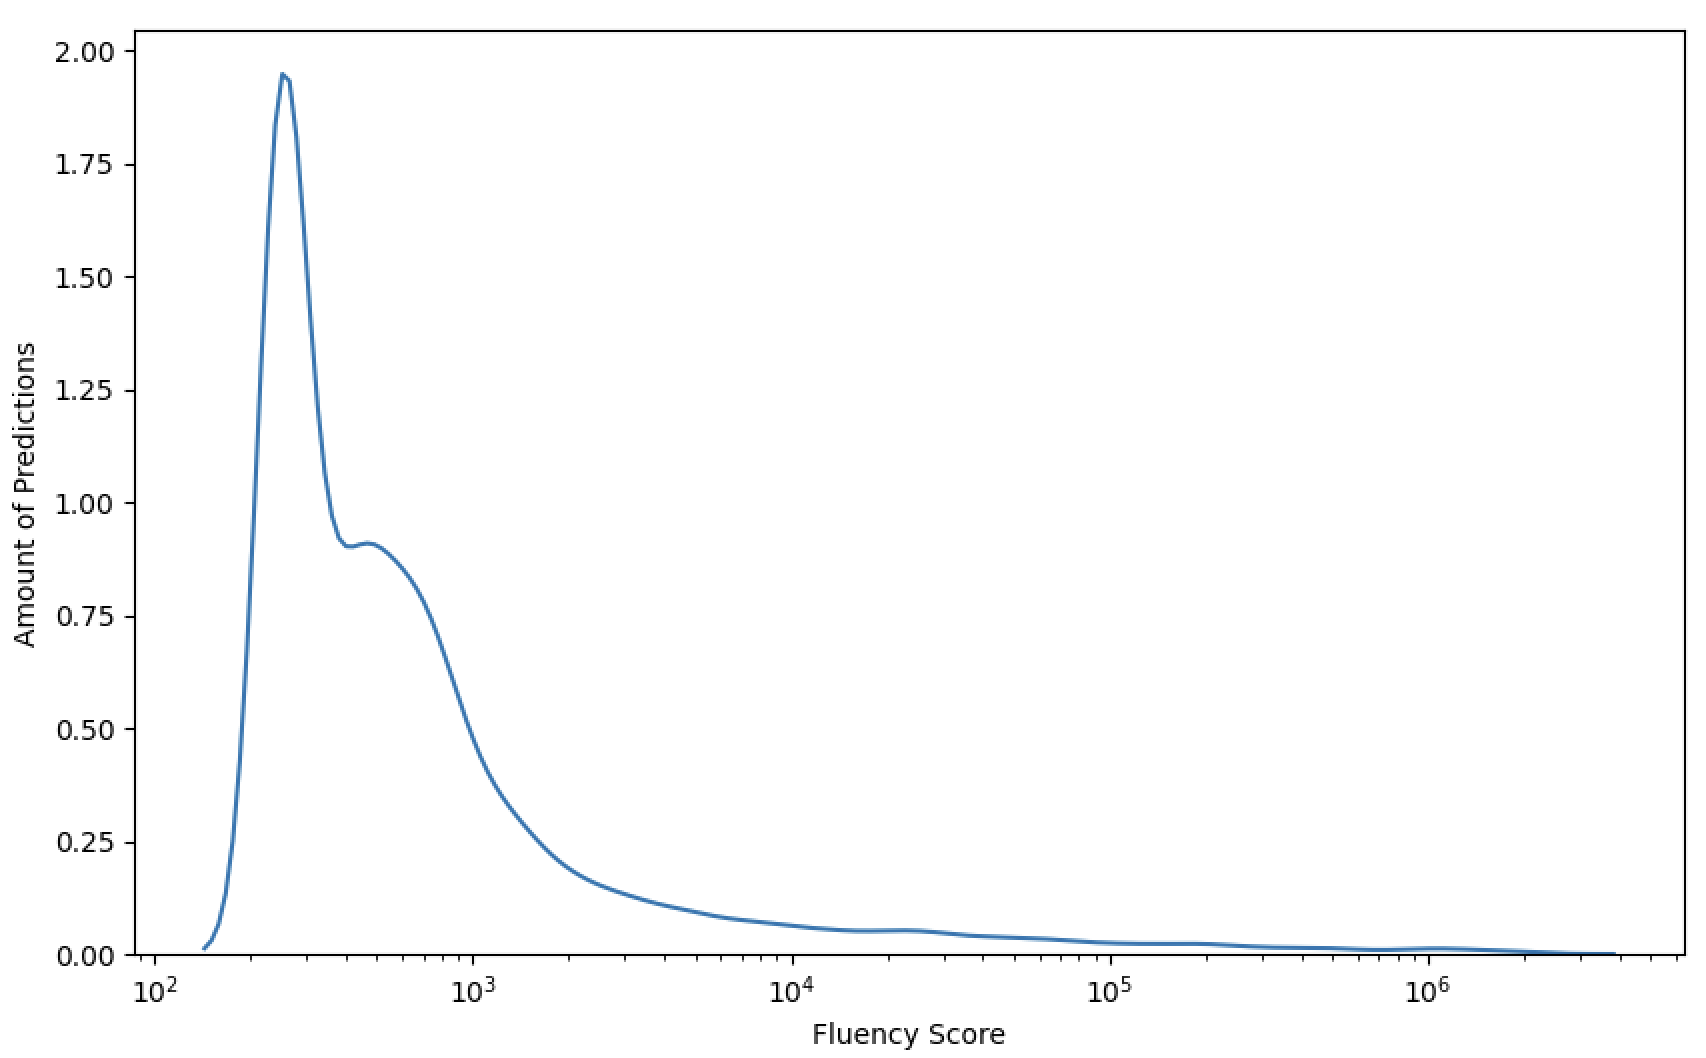
\includegraphics[width=0.7\textwidth]{KDE_score.png}
    \caption{Kernel density estimate of fluency score}
    \label{fig:word_freq}
\end{figure}

Table \ref{tab:Score_stats} shows the summary statistics of the predicted fluency score. 

\begin{table}[htbp]
\centering
\caption{Summary statistics of fluency score prediction}
\label{tab:Score_stats}
\begin{tabular}{ll}
\toprule
\textbf{Statistic} & \textbf{Value} \\
\midrule
Mean & 12167.150 \\
Median & 445.826 \\
Minimum & 241.034 \\
Maximum & 2277662.000 \\
Standard Deviation & 98788.601 \\
\bottomrule
\end{tabular}
\end{table}
\newpage
\section*{Appendix C: Tuned Hyperparameters}\label{Appendix C}
Table~\ref{tab:hyperparameters} provides an overview of the tuned hyperparameters. The \textbf{Structure} column shows the corresponding layer, while the \textbf{Hyperparameter} column lists the settings applied, such as activation functions, regularisation, and dropout. The final column presents the selected values. The bottom section of the table summarizes global network-level settings.

\begin{table}[htbp]
\begin{center}
\caption{Tuned hyperparameters of the deep learning model}
\label{tab:hyperparameters}
\begin{tabular}{llllcl}
\toprule
\textbf{Structure} & & \textbf{Hyperparameter} & & \textbf{Value} & \\ \midrule

Layer 1 && Amount of nodes && 32 & \\
        && Activation function && Sigmoid & \\
        && Regularisation type && None & \\
        && Regularisation rate && 0.0 & \\
        && Batch Normalisation applied && No & \\
        && Dropout applied && No & \\
        && Dropout rate && 0.2 & \\

Layer 2 && Amount of nodes && 16 & \\
        && Activation function && Sigmoid & \\
        && Regularisation type && L1\_L2 & \\
        && Regularisation rate && 0.0 & \\
        && Batch Normalisation applied && No & \\
        && Dropout applied && Yes & \\
        && Dropout rate && 0.1 & \\

Layer 3 && Amount of nodes && 16 & \\
        && Activation function && Sigmoid & \\
        && Regularisation type && L2 & \\
        && Regularisation rate && 0.0 & \\
        && Batch Normalisation applied && Yes & \\
        && Dropout applied && No & \\
        && Dropout rate && 0.2 & \\

Layer 4 && Amount of nodes && 4 & \\
        && Activation function && Sigmoid & \\
        && Regularisation type && None & \\
        && Regularisation rate && 0.001 & \\
        && Batch Normalisation applied && No & \\
        && Dropout applied && Yes & \\
        && Dropout rate && 0.1 & \\

Layer 5 && Amount of nodes && 32 & \\
        && Activation function && ReLU & \\
        && Regularisation type && L1\_L2 & \\
        && Regularisation rate && 0.01 & \\
        && Batch Normalisation applied && No & \\
        && Dropout applied && No & \\
        && Dropout rate && 0.2 & \\

Layer 6 && Amount of nodes && 16 & \\
        && Activation function && ReLU & \\
        && Regularisation type && None & \\
        && Regularisation rate && 0.01 & \\
        && Batch Normalisation applied && Yes & \\
        && Dropout applied && No & \\
        && Dropout rate && 0.2 & \\

\midrule
Network && Amount of hidden layers && 4 & \\
        && Learning rate && 0.0001 & \\
        && Epochs && 20 & \\
\bottomrule
\end{tabular}
\end{center}
\end{table}



\end{document}